% !TEX root = .

\documentclass[a4paper, 12pt, oneside, BCOR1cm,toc=chapterentrywithdots, hidelinks]{scrbook}
\usepackage{scrhack}

\usepackage[a4paper]{geometry}
\usepackage{textcomp}
\usepackage{longtable}
\usepackage{tabularx}
%\usepackage{tabu}

\usepackage[ngerman, english]{babel}
\usepackage[utf8]{inputenc}
\usepackage{graphicx} 
\usepackage{acronym}
\usepackage{url}           	 
\usepackage{hyperref} 	
\usepackage{listings, color}	% for source code
\usepackage{scrlayer-scrpage}	% header and footer line
\usepackage{acronym}
\usepackage[ruled,vlined,algochapter]{algorithm2e}
%\usepackage[nottoc, notlof, notlot]{tocbibind}
\usepackage{blindtext}

\usepackage{chngcntr}
\counterwithout{figure}{chapter}
\counterwithout{table}{chapter}
\counterwithout{algocf}{chapter} 
%\counterwithout{lstlisting}{chapter}
\AtBeginDocument{% the counter is defined later
  \counterwithout{lstlisting}{chapter}%
}
\renewcommand\lstlistingname{Code Fragment}

%for adding comments
\usepackage{verbatim}

% for tables
\usepackage{multirow}
\usepackage[table]{xcolor}
\usepackage{xcolor}

% header and footer line - no header & footer line on pages where a new chapter starts
\pagestyle{scrheadings}
% TU Berlin logo at header
%\chead{
\includegraphics[width=1.2cm]{./img/TU-Berlin-Logo.pdf} 
%}



\begin{document}

\frontmatter
%Titlepage
\thispagestyle{empty}
\begin{center}

\begin{figure}[t]
    \centering
    
\includegraphics[width=3cm]{./img/TU-Berlin-Logo.pdf}%
%    \qquad
%    \includegraphics[width=3.3cm]{dima_logo.png}%
\end{figure}

%\vspace*{0.2cm}
{\LARGE \textbf{Technische Universit\"at Berlin}}

\vspace{0.5cm}

{\large Chair of Database Systems and Information Management\\[1.6mm]}
%{\large Fachgebiet Datenbanksysteme und Informationsmanagement\\[5mm]}

%Fakult\"at IV\\
%Einsteinufer 17\\
%10587 Berlin\\
%https://www.dima.tu-berlin.de\\

\vspace{2.0cm}

{\LARGE Master's Thesis}\\

\vspace{2.45cm}
{\LARGE \textbf{Anonymized Access Control for Distributed Event Stores}}\\
%\vspace*{0.3cm}
%{\LARGE \textbf{second Line}}\\
\vspace{1.0cm}
%{\LARGE Firstname Lastname(s)}
%\vspace*{0.5cm}
Henri Tyl Allgöwer \\
Degree Program: Computer Science\\
Matriculation Number: 454925\\

\vspace*{2.45cm}
\textbf{Reviewers}\\
Prof. Dr. Volker Markl\\
Prof. Dr. Odej Kao\\
\vspace*{0.5cm}
\textbf{Advisor}\\
Rudi Poepsel Lemaitre\\
\vspace{0.5 cm}

\textbf{Submission Date}\\
30.11.2023\\ % 	date of submission
\end{center}


\thispagestyle{empty}
\cleardoublepage
    
%Self-assertion
\newpage

\thispagestyle{empty}

\begin{large}

\vspace*{6cm}

\noindent
Hereby I declare that I wrote this thesis myself with the help of no more than the mentioned literature and auxiliary means.
\vspace{2cm}

\noindent
Berlin, \today

\vspace{3cm}

\hspace*{7cm}%
\dotfill\\
\hspace*{7.5cm}%
\textit{Henri Tyl Allgöwer}

\end{large}
 
\thispagestyle{empty}
\cleardoublepage

% Abstract in Deutsch
\addchap*{Zusammenfassung}
Tipps zum Schreiben dieses Abschnitts finden Sie unter \cite{wallwork_177}

% Abstract
\addchap*{Abstract}
Modern database systems are of incredible importance. Without them, our entire infrastructure would fall apart. Hospitals could no longer properly treat patients, lacking the necessary patient records and treatment history. Banks and financial services would be left unable to execute transactions. Telecommunication services would shut down. These modern database systems often utilize message brokers in combination with stream processing engines. They are capable of accumulating, processing, and distributing data in real-time at an unprecedented rate and volume. With the focus firmly on performance and scalability, data protection has been left behind. A critical oversight as protecting sensitive data is essential in ensuring personal privacy, preventing misuse and fraud, and upholding trust in data handling. At the moment, these database systems provide only very basic access control and lack mechanisms for enforcing privacy policies. Companies often resort to encrypting the data flowing through database systems and focus on external authentification and authorization. Processing encrypted data, however, comes with challenges including computational overhead, added complexity, and performance trade-offs. Decrypting the data again before processing leads back to square one. \par
This thesis introduces a novel model for data anonymization with integrated access control enforcing mechanisms uniquely within modern database systems, more specifically \acfp{DES}. We have realized our model through the development of a new system the \acf{DASH} for Apache Kafka, a leading \ac{DES}. \ac{DASH} is capable of applying a broad variety of anonymization techniques to data streams, uniquely within the database infrastructure. Our tests demonstrate \ac{DASH}'s ability to apply anonymization on individual tuples without introducing performance overhead. We found more complex anonymization techniques, such as those required for achieving k-anonymity on collections of tuples, to be strongly coupled with available system resources. Our evaluation reveals that simpler anonymization techniques are suited for even the highest performance demands, whereas more complex anonymization techniques are more limited in their application.
  
% Acknowledgments  
\addchap*{Acknowledgments}
For recommendations on writing your Acknowledgments see \cite{wallwork_306}.
Thank you to the chair at \ac*{DIMA}

%table of contents
\addtocontents{toc}{\protect\setcounter{tocdepth}{-1}}
\tableofcontents
\addtocontents{toc}{\protect\setcounter{tocdepth}{3}}

%footnote
\newcommand\blfootnote[1]{%
  \begingroup
  \renewcommand\thefootnote{}\footnote{#1}%
  \addtocounter{footnote}{-1}%
  \endgroup
}
\blfootnote{Chapters 3-5 are the core of the thesis, whereas Chapters 1, 2, 6, and 7 provide context. The major contributions should be in Chapters 4 and 5. This structure serves as a guideline and should be customized accordingly. In particular, the generic chapter titles should be replaced with more specific ones, where appropriate (e.g., Chapter 4).} 

%list of figures
\listoffigures

%list of tables
\listoftables



    

    

% List of Abbreviations
\onecolumn
\addchap{List of Abbreviations}
\begin{acronym}[Bash]   
 \acro{DIMA}{Database Systems and Information Management}
 \acro{CCPA}{California Consumer Privacy Act}
 \acro{GDPR}{General Data Protection Regulation}
 \acro{ICD}{International Statistical Classification of Diseases and Related Health Problems}
\end{acronym}
\onecolumn


%algorithms
\listofalgorithms
\addcontentsline{toc}{chapter}{List of Algorithms}

%In case, code fragments have to be added
%\renewcommand{\lstlistlistingname}{List of Code Fragments}
%\lstlistoflistings
%\addcontentsline{toc}{chapter}{List of Code Fragments}

\mainmatter % comment single chapters for faster compilation
    
    \chapter{Introduction\label{cha:chapter1}}
Distributed event stores capture, store, and process real-time data streams in distributed environments. They have been widely adopted across various sectors, including Fortune 100 companies, governments, healthcare, and transportation industries \cite{kafka} for their efficient, scalable, and fault-tolerant system design. In the modern data-driven world, the growing demand for comprehensive data privacy policies has resulted in increasingly stringent regulations from governments worldwide \cite{GDPR, CCPA}. However, the underlying infrastructure for distributed event stores to adequately support these policies is markedly lacking \cite{Colombo2015}. This disparity poses a unique challenge, particularly when considering the demands of modern database systems to maintain high performance, characterized by low latency and high throughput.\par
The present work aims to examine what techniques can be effectively employed to ensure privacy and security measures, such as access control and data masking, in distributed event stores. Additionally, it aims to explore what strategies can be developed and implemented to ensure that these privacy and security measures have a minimal impact on the performance of distributed event stores. \par
While there exists a body of work focusing on anonymization and data masking for data streaming \cite{Cao2008, KIDS_zhang, anonymizing_IoT}, there is a noticeable gap in research specifically targeting distributed event stores. 
Furthermore, although there are enterprise technologies for managing data flowing into such systems \cite{privitar}, there is limited literature on techniques designed for data already within distributed event stores. Most notably, the concept of integrating \ac{RBAC} within this framework, where the role assigned determines the level of anonymity accorded to the data, is a completely novel approach. \par
The introduction of access control coupled with anonymization in distributed event stores holds the potential to contribute to more advanced, efficient, and secure data handling. By making such tools accessible and cost-effective, companies might be more inclined to prioritize and invest in user data privacy.\par
The overarching goal of this thesis is to design, implement, and evaluate a management framework for distributed event stores. This framework aims to incorporate \ac{RBAC}, granting administrators the capacity to define levels of data anonymization and specify masking functions. By associating levels of anonymization with the number of additional data streams per original data stream, the framework will facilitate nuanced and customizable data privacy measures. Moreover, this plugin will facilitate the assignment of consumers to streams based on their specific roles, further enhancing granular control over data access and privacy within distributed event stores.\par
The scope of this thesis will primarily encompass the exploration of privacy and security measures in the context of distributed event stores. The thesis will delve into the administrative aspects of these technologies, including the implementation and management of access control and data masking functions. Particular attention will be paid to the role of administrators and the impact of their decisions on the performance of these systems. This includes the computational implications of various anonymization techniques. It will involve an in-depth study of different strategies' performance impacts, aiming to minimize overhead while maintaining robust data privacy. At the same time, this thesis will not specifically address or align with any particular data privacy policy such as the \ac{GDPR} \cite{GDPR}. While the thesis is designed around general principles of data privacy and security, it will not provide policy-specific solutions or address the nuances of any specific regulatory framework. Furthermore, the anonymization of data flowing into or out of distributed event stores is beyond the scope of this thesis. The focus will primarily be on the data within the systems, and not on the methods and protocols for handling data entering or leaving these systems. \par
This thesis introduces the \acf{DASH}, a system architected to process data streams into multiple anonymized versions. This design aims to provide users of distributed event stores with a nuanced granularity of anonymization. A comprehensive survey of anonymization techniques is presented, categorizing these methodologies for practical application in various scenarios. \ac{DASH} includes an extensive library of anonymization techniques, offering users the flexibility to tailor the anonymization process to their specific requirements. Additionally, role-based access control is made available as a separate component to assign anonymized versions to streams. This combination of access control with anonymization variety is not only theoretically robust but also practically applicable. Its synergy is highlighted in our theoretical framework chapter, where we showcase a real-world example. Furthermore, this thesis presents a theoretical model designed to simplify future implementations of anonymized access control across various distributed event stores. \par
In the context of this research, we have tested and evaluated \ac{DASH} in an extensive data pipeline environment. We have found \dots \par
The thesis is structured as follows: in Chapter \ref{cha:chapter2} we conduct a literature review. The theoretical framework is constructed in Chapter \ref{cha:chapter3}. Subsequently, Chapter \ref{cha:chapter4} examines in detail the implementation. Tests and their evaluations are addressed in Chapter \ref{cha:chapter5}. Finally, Chapter \ref{cha:chapter6} presents the conclusion and offers an outlook on future work.

    \chapter{Literature Review\label{cha:chapter2}}

\section{Distributed Event Stores}

\section{Anonymization\label{sec:anon}}

\section{Role Based Access Control}

\section{Privitar}

... should include the following:
\begin{itemize}
    \item definitions / technical terms,
    \item theoretical foundations / principles,
    \item descriptions of algorithms, hardware, software, and/or systems employed.
\end{itemize}



\begin{figure}[h]
\centering
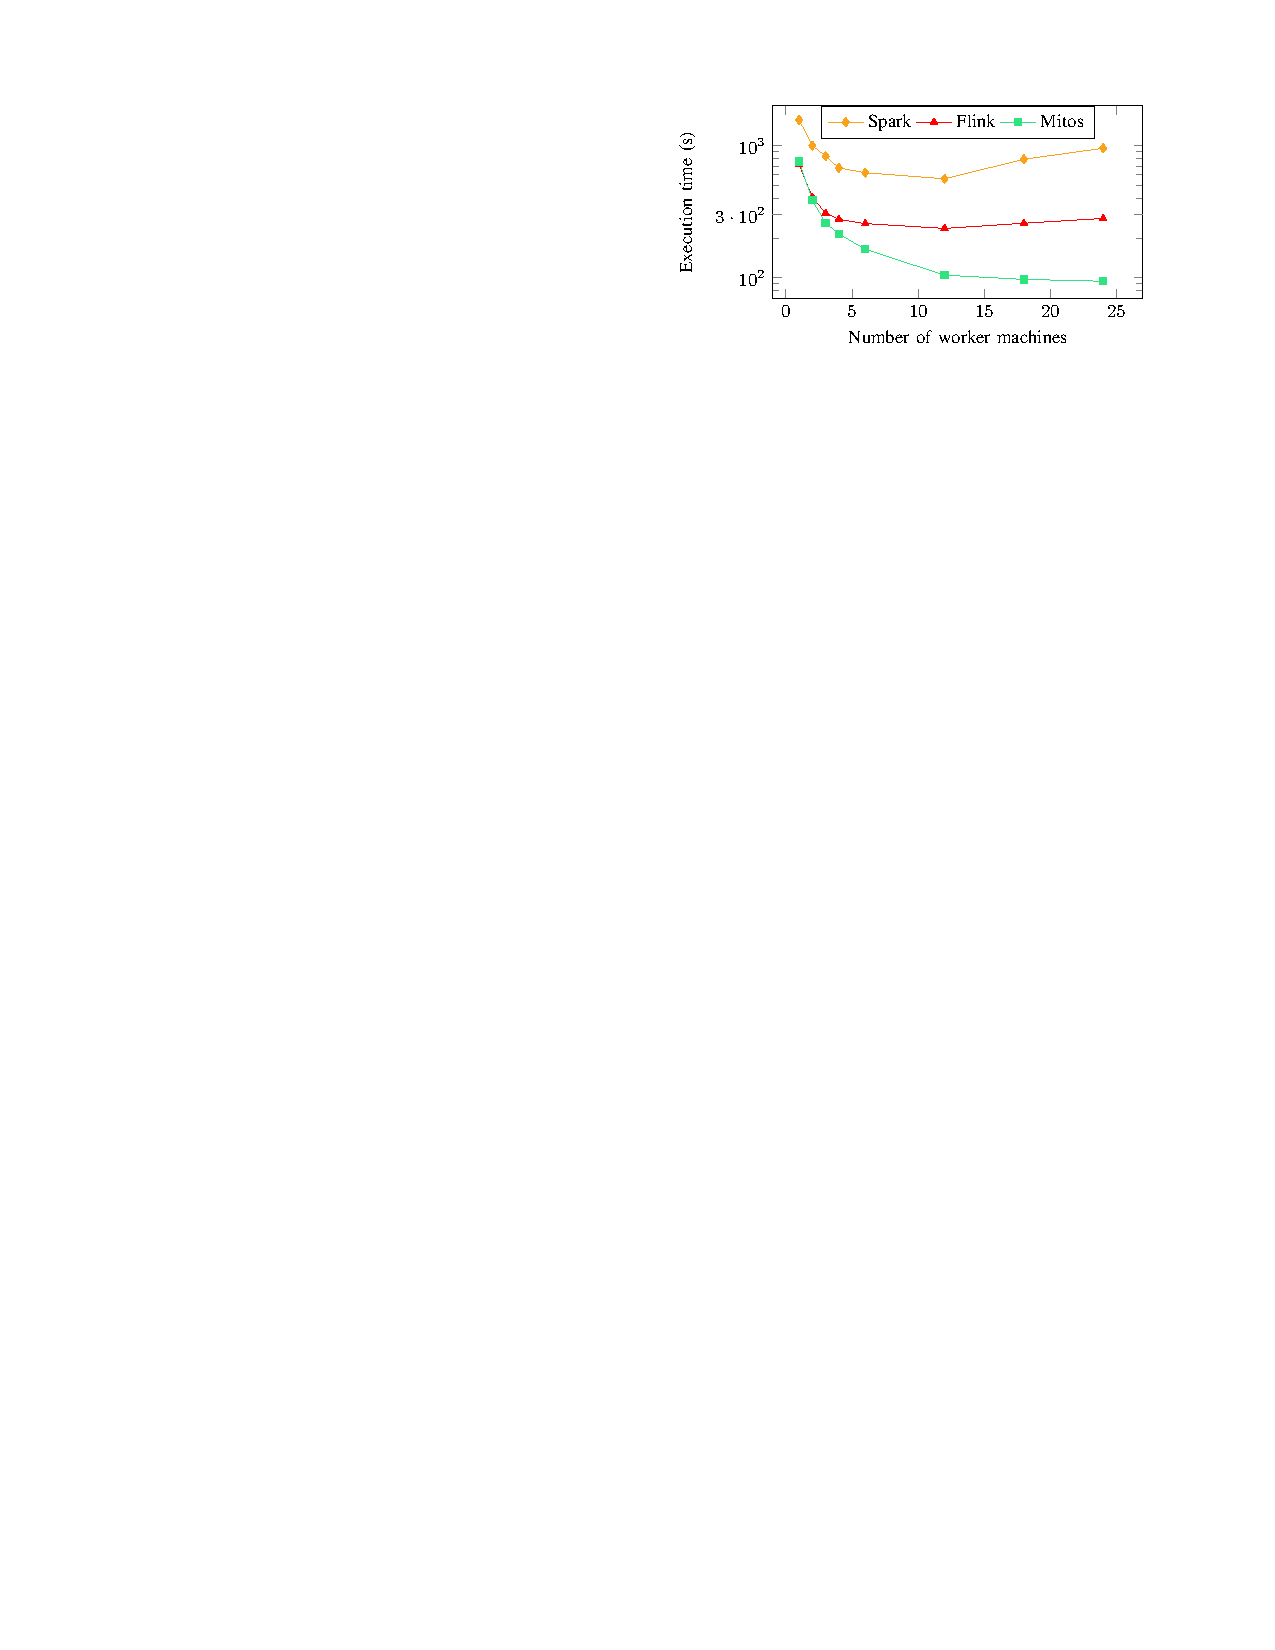
\includegraphics[width=0.6\textwidth]{./img/strong_scaling.pdf}
\caption{Strong scaling for Visit Count\cite{GevayRBMQM21}.}
\end{figure}

% We can leave this out... The advisor can point this out, if it is a concern.
%Suggestion: Figures could be inserted in pdf form to avoid pixelation when the image is magnified.

%This section is intended to give an introduction about relevant terms, technologies and standards in the field of X. You do not have to explain common technologies such as HTML or XML. 



    \chapter{Theoretical Framework\label{cha:chapter3}}

\section{Managing Different Anonymization Granularity}
When planning to integrate anonymization techniques into existing systems, there are many things to consider. First one must understand the data flowing through the system.
Does it include \ac{PII}? Is there further sensitive data? What part of it is necessary for system maintenance? Maybe there is additional data collected for statistics.
Bearing this in mind the next thought would what needs to be anonymized. For this privacy agreements with the user must be taken into account. There may be additional government regulations in place like the \ac{CCPA} in the United States of America or the \ac{GDPR} in the European Union. 
The next course of action is deciding on specific masking functions. As was discussed in \ref{sec:anon} there is a plethora to chose from. It is important to note that all forms of anonymization lead to a loss of information. 
While choosing Blurring or Suppression, two methods that replace attributes with a placeholder, for all critical data fields derived in the previous assessment will ensure that all privacy concerns are addressed, it will also diminish all intelligence gained from collecting this data in the first place. It is questionable if not collecting this type of data in the first place would then be the better solution as it would save storage and computing power. 
An alternative approach would be to invest heavily in the IT security ensuring that no intruder with malicious intent can gain access to sensitive data. Keeping in mind, however, that social engineering attacks are nowadays the most common and effective strategy (SAUCE) giving a guarantee of safety can be impossible. It also stands to reason that the more employees a company has the risk for social
engineering attacks increases. Both of these radical approaches do not seem to adequately solve the problem. Fortunately, there is a way to navigate between these two extremes. An attentive observer of the company's data operations will likely notice that data can and should be restricted similarily to permissions: Only the data needed to furfill the user's duty should be accessible to the user. 
In addition, there are anonymization techniques, which do not lead to total information loss like the two mentioned before. Generalization for example can be employed to significantly reduce the re-identification of individuals, while simultaneously retaining some information.
With data restriction and different anonymization techniques in mind there is a middle ground to be found which maximizes security and minimizes information loss. Consider the following example:

\subsection{Use Case Example}
Hospitals depend on the collection, management and analysis of data to administer the best and most accurate care of their patients. In a modern hospital all data would be stored in a centralized hospital database. 
Here all data for individual patients are brought together. Table \ref{table:dia_patient} shows an exemplary table of patients in the endocrinology ward of a german hospital. Note that the tuple has been shortened to enhance its readability as well as prepended with a header of the corresponding database table.  (A MORE DETAILED VERSION CAN BE FOUND IN THE APPENDIX)


\bigskip 


\begin{table}[ht]
    \begin{center}
    \footnotesize{
        \renewcommand{\arraystretch}{1.5}
        \begin{tabular}{ | c | c | c | c | c | c | c | c | c | c | c | } 
            \hline
            pid & name & zip & sex & age & ins. co. & ins. no. & diag. & gluc. & hba1c & med. \\
            \hline
            1 & F. Ott & 10969 & M & 28 & TK & K15489 & E10 & 22.1 & 8.74 & Insulin \\
            \hline
            2 & L. Lieb & 34127 & F & 59 & AOK & Y41271 & E11 & 16.3 & 7.61 & Metformin \\
            \hline 
            3 & T. Zeit & 70192 & M & 15 & TK & Z17291 & E10 & 23.8 & 8.13 & Insulin \\
            \hline
            4 & H. Lang & 80923 & F & 21 & TK & I79435 & E10 & 18.9 & 7.99 & Insulin \\
            \hline
            5 & J. Putz & 91757 & D & 24 & IKK & Q29751 & E10 & 21.2 & 6.04 & Insulin \\
            \hline
            6 & I. Spies & 60819 & M & 68 & TK & J33921 & E11 & 19.1 & 5.07 & Metformin \\
            \hline
        \end{tabular}
    }
    \caption{Example table of diabetes patients}
    \label{table:dia_patient}
    \end{center}
\end{table}

The header of table \ref{table:dia_patient} shows eleven attributes. First the person id (\textit{pid}), which is the primary key for each patient as it uniquely identifies the patient in the database. Then \textit{name}, zip code (\textit{zip}), \textit{sex} and \textit{age} are included as additional personal information.
This would typically also include the full address not just the zip code, contact information, height as well as weight to adapt the dosage of the medication. The subsequent two attributes include information about the patient's insurance information. 
Insurance companies in Germany are uniquely identified with a nine digit institutional identifier. In the case of the first entry the insurance company (\textit{ins. co.}) has the value 101575519, which matches the identifier of the Techniker Krankenkasse (TK). 
Each client is then assigned a number unique to that insurance company called the insurance number (\textit{ins. no.}). It always starts with a letter followed by digits. Finally, the datum references the medical information. It starts with the diagnosis (\textit{diag.}) classified according to the \ac*{ICD}. 
E10 being the label for Type 1 Diabetes Mellitus, E11 the label for Type 2 Diabetes Mellitus. The most important medical measurement for the treatment of this disease is the current amount of glucose (\textit{gluc.}) in the blood. This determines the quantity of medication (\textit{med.}) to be administered to the patient. For Type 1 Diabetes this is Insulin, for Type 2 it is Metformin. 
Lastly, the table includes an attribute called \textit{hba1c}. This is the body's own three-month average of blood glucose. By means of which diabetes is diagnosed. In this case it is also symbolic for all additional diagnostic findings. 
Glucose and HbA1c are intentionally distinguished as separate attributes in this dataset, despite both being blood-derived metrics, due to their distinct measurement methodologies and relevance in immediate treatment contexts. Glucose can be ascertained with a single drop of blood, providing critical information for the immediate treatment.
Conversely, HbA1c is derived from a complete blood count and does not require instant action. \newline

In a hospital setting, numerous actors engage with the aforementioned dataset. The most straightforward and prominent is the doctor. She will need all data to fulfill her duties. The doctor's letter contains all personal information. The medical data is needed for diagnosis and treatment. 
She will also need to keep the insurance information in mind as the covered treatment options are oftentimes different for each company. Additionally, she will need to write the patient's insurance information on the rescriptions. Only the pid could be omitted, but is debatable if the overhead is worth it, considering the pid can be easily inferred with all the given information.
Therefore, no anonymization to the doctor's data makes the most sense. \\\\
\indent Supporting the doctor is the nurse staff. One of their main tasks is to monitor patients and administer medication. To accomplish this they require the diagnosis, medication and in this case the glucose data. As the HbA1c value is not relevant for the immediate treatment it can be safely ommitted. 
Again insurance information is necessary as nurses typically do have the liberty of administer medication according to their own judgement. This is especially important when considering how understaffed hospitals in Germany are most of the time. On the other hand the patient's personal insurance number does not play into this. As nurses also interact directly with the patients they need some basic personal information like name and sex. 
Pid and zip, however, are not required. Therefore, the data for the nurse staff can be anonymized as shown in Table \ref{table:nurse} without limiting the nurses or losing valuable information. 

\bigskip

\begin{table}[ht]
    \begin{center}
    \footnotesize{
        \renewcommand{\arraystretch}{1.5}
        \begin{tabular}{ | c | c | c | c | c | c | c | c | c | c | c | } 
            \hline
            \cellcolor{lightred} pid & name & \cellcolor{lightred} zip & sex & age & ins. co. & \cellcolor{lightred} ins. no. & diag. & gluc. & \cellcolor{lightred} hba1c & med. \\
            \hline
            \cellcolor{lightred} * & F. Ott & \cellcolor{lightred} * & M & 28 & TK & \cellcolor{lightred} * & E10 & 22.1 & \cellcolor{lightred} * & Insulin \\
            \hline
            \cellcolor{lightred} * & L. Lieb & \cellcolor{lightred} * & F & 59 & AOK & \cellcolor{lightred} * & E11 & 16.3 & \cellcolor{lightred} * & Metformin \\
            \hline 
            \cellcolor{lightred} * & T. Zeit & \cellcolor{lightred} * & M & 15 & TK & \cellcolor{lightred} * & E10 & 23.8 & \cellcolor{lightred} * & Insulin \\
            \hline
            \cellcolor{lightred} * & H. Lang & \cellcolor{lightred} * & F & 21 & TK & \cellcolor{lightred} * & E10 & 18.9 & \cellcolor{lightred} * & Insulin \\
            \hline
            \cellcolor{lightred} * & J. Putz & \cellcolor{lightred} * & D & 24 & IKK & \cellcolor{lightred} * & E10 & 21.2 & \cellcolor{lightred} * & Insulin \\
            \hline
            \cellcolor{lightred} * & I. Spies & \cellcolor{lightred} * & M & 68 & TK & \cellcolor{lightred} * & E11 & 19.1 & \cellcolor{lightred} * & Metformin \\
            \hline
        \end{tabular}
    }
    \caption{Data available for the nurse staff. Note that pid, zip, insurance number and additional medical information have been suppressed as indicated by their cell's light red background.}
    \label{table:nurse}
    \end{center}
\end{table}

In tandem with the stay and medical treatment of the patient, the administartion of the hospital will want to collect the money from the patient's insurance. The insurance company together with the patient's personal insurance number will suffice as identification. 
Administered medication will be imperative as this dictates the amount of money the hospital will get in addition to the fees for the stay. For this the diagnosis will typically have to be added as a suitable reason. No further information is required. Limiting the amount of data here 
is crucial as here the data is exported to a third party. Which means that additional regulations will take effect. Minimizing the data leaving the hospital minimizes security risks. With these strict rules in place the data can be adjusted as seen in Table \ref{table:administration}. \newline 
Note at this point that an unauthorized entity, who has gained access to both the data of the nurse staff and that of the administration, would struggle to correlate the entries. The shared available data fields insurance company, diagnosis and medication are likely generic enough to not point to a singular but to many patients. 

\bigskip

\begin{table}[ht]
    \begin{center}
    \footnotesize{
        \renewcommand{\arraystretch}{1.5}
        \begin{tabular}{ | c | c | c | c | c | c | c | c | c | c | c | } 
            \hline
            \cellcolor{lightred} pid & \cellcolor{lightred} name & \cellcolor{lightred} zip & \cellcolor{lightred} sex & \cellcolor{lightred} age & ins. co. & ins. no. & diag. & \cellcolor{lightred} gluc. & \cellcolor{lightred} hba1c & med. \\
            \hline
            \cellcolor{lightred} * & \cellcolor{lightred} * & \cellcolor{lightred} * & \cellcolor{lightred} * & \cellcolor{lightred} * & TK & K15489 & E10 & \cellcolor{lightred} * & \cellcolor{lightred} * & Insulin \\
            \hline
            \cellcolor{lightred} * & \cellcolor{lightred} * & \cellcolor{lightred} * & \cellcolor{lightred} * & \cellcolor{lightred} * & AOK & Y41271 & E11 & \cellcolor{lightred} * & \cellcolor{lightred} * & Metformin \\
            \hline 
            \cellcolor{lightred} * & \cellcolor{lightred} * & \cellcolor{lightred} * & \cellcolor{lightred} * & \cellcolor{lightred} * & TK & Z17291 & E10 & \cellcolor{lightred} * & \cellcolor{lightred} * & Insulin \\
            \hline
            \cellcolor{lightred} * & \cellcolor{lightred} * & \cellcolor{lightred} * & \cellcolor{lightred} * & \cellcolor{lightred} * & TK & I79435 & E10 & \cellcolor{lightred} * & \cellcolor{lightred} * & Insulin \\
            \hline
            \cellcolor{lightred} * & \cellcolor{lightred} * & \cellcolor{lightred} * & \cellcolor{lightred} * & \cellcolor{lightred} * & IKK & Q29751 & E10 & \cellcolor{lightred} * & \cellcolor{lightred} * & Insulin \\
            \hline
            \cellcolor{lightred} * & \cellcolor{lightred} * & \cellcolor{lightred} * & \cellcolor{lightred} * & \cellcolor{lightred} * & TK & J33921 & E11 & \cellcolor{lightred} * & \cellcolor{lightred} * & Metformin \\
            \hline
        \end{tabular}
    }
    \caption{Data available for the administration. Note that only the insurance information, medication and diagnosis are not suppressed.}
    \label{table:administration}
    \end{center}
\end{table}

Diabetes, which afflicts over ten percent of the global population and demonstrates a rising prevalence, stands as one of the most common chronic diseases worldwide \cite{idf2023,WHODiabetes2023}. Given its mostly non-lethal progression and lifetime dependency on medication, 
it has given rise to a substatial market. As cause, optimal treatment and cure remain subject to research, data of especially newer diabetes patients is in hot demand. To provide this data to research institutes in accordance with the regulations in place the hospital must ensure that no concrete patient can be reidentified. 
Here, advanced anonymization techniques such as K-Anonymization come into place. Each attribute of the data entry can be assigned to one of three categories: personally identifiable, quasi identifying and sensitive attributes. To achieve k anonymity each entry must suppress the personally identifiable attributes, while keeping the sensitive attributes untouched. 
Most importantly the quasi identifiable attributes of each data entry must be the same for at least k - 1 other entries of a data set. This is typically achieving with generalization of these attributes until k entries are found. In this use case the personally identifiable attributes are \textit{pid}, \textit{name} and \textit{insurance number}. 
The quasi indentifying attributes are \textit{zip}, \textit{sex}, \textit{age} and \textit{insurance company}. The medical data comprive the sensitive attributes. A K anonymous version of this data extry is depicted in Table \ref{table:k_anon}. 

\bigskip

\begin{table}[ht]
    \begin{center}
        \footnotesize{
            \renewcommand{\arraystretch}{1.5}
            \begin{adjustbox}{center}
                \begin{tabular}{ | c | c | c | c | c | c | c | c | c | c | c | } 
                    \hline
                    \cellcolor{lightred} pid & \cellcolor{lightred} name & \cellcolor{lightyellow} zip & \cellcolor{lightyellow} sex & \cellcolor{lightyellow} age & \cellcolor{lightyellow} ins. co. & \cellcolor{lightred} ins. no. & diag. & gluc. & hba1c & med. \\
                    \hline
                    \cellcolor{lightred} * & \cellcolor{lightred} * & \cellcolor{lightyellow} XXXXX & M & \cellcolor{lightyellow} {[10 - 70]} & TK & \cellcolor{lightred} * & E10 & 22.1 & 8.74 & Insulin \\
                    \hline
                    \cellcolor{lightred} * & \cellcolor{lightred} * & \cellcolor{lightyellow} XXXXX & M & \cellcolor{lightyellow} {[10 - 70]} & TK & \cellcolor{lightred} * & E10 & 23.8 & 8.13 & Insulin \\
                    \hline 
                    \cellcolor{lightred} * & \cellcolor{lightred} * & \cellcolor{lightyellow} XXXXX & M & \cellcolor{lightyellow} {[10 - 70]} & TK & \cellcolor{lightred} * & E11 & 19.1 & 5.07 & Metformin \\
                    \hline
                    \cellcolor{lightred} * & \cellcolor{lightred} * & \cellcolor{lightyellow} XXXXX & \cellcolor{lightyellow} \{M, F, D\} & \cellcolor{lightyellow} {[10 - 70]} & \cellcolor{lightyellow} ins. co & \cellcolor{lightred} * & E11 & 16.3 & 7.61 & Metformin \\
                    \hline
                    \cellcolor{lightred} * & \cellcolor{lightred} * & \cellcolor{lightyellow} XXXXX & \cellcolor{lightyellow} \{M, F, D\} & \cellcolor{lightyellow} {[10 - 70]} & \cellcolor{lightyellow} ins. co & \cellcolor{lightred} * & E10 & 18.9 & 7.99 & Insulin \\
                    \hline
                    \cellcolor{lightred} * & \cellcolor{lightred} * & \cellcolor{lightyellow} XXXXX & \cellcolor{lightyellow} \{M, F, D\} & \cellcolor{lightyellow} {[10 - 70]} & \cellcolor{lightyellow} ins. co & \cellcolor{lightred} * & E10 & 21.2 & 6.04 & Insulin \\
                    \hline
                \end{tabular}
            \end{adjustbox}
        }
    \caption{K-anonymized data available for external research. The sensitive medical attribtues remains unchanged as indicated by the white cell background. Unlike the personally identifying attributes, which have been suppressed as denoted by the red cell background. The yellow cell background highlights the generalized quasi identifiable attributes. Note that the entries of the first group have unchanged values for the attributes \textit{sex} and \textit{ins. co.}. As all three original entries shared the same value it did not need to be generalized.}
    \label{table:k_anon}
    \end{center}
\end{table}

While the aforementioned diabetes patient use case scenario may appear unique and specific, the aspects and nuances are applicable in numerous contexts. The distinct data requirements for doctors, nurses, administration and research are anticipated to persist, albeit adapted, throughout the entire healthcare industry. 
It is also viable in different sectors. Imagine security levels in government matters, trade secrets and specific customer knowledge in corporations or secrecy of correspondense for the transportation industry. Distributed event stores are utilized across all of these sectors with major players relying on Apache Kafka for their day to day needs \cite{KafkaPoweredBY}. 

\section{Anonymization Techniques}
Data anonymization is a multifaceted process tailored to meet application requirements, user groups and their specific needs. This section first goes in depth into masking functions, the cornerstone of data anonymization. It then explores table based techniques that look at the whole dataset to ensure privacy. In this context a \textit{datum} refers to a single piece of information e.g. a singular entry of a database or any one event of a data stream. Synonymous with it also used the word \textit{tuple}. A tuple is comprived of one or multiple \textit{attributes} (also called \textit{fields}). It is customary for individual tuples to be part of a bigger collection. In the static context they are collected in databases and grouped in tables. Data streams work analogous for dynamic operations. All tuples of the same database table or data stream are required to follow the same pattern. This refers to the sequence of attributes of each tuple. This pattern is fixed in a data schema associated with the table or stream. Sometimes it is appended to each datum in form of a header as seen exemplary in Table \ref{table:dia_patient}. As this substantially increases the size of each datum it is more common to define it once in the initialization step of the database table or data stream. \\
While all forms of anonymization aim to alter the underlying sensitive information, e.g. the tuple's attributes containing perhaps personally identifiying information, in a way that makes it harder if not impossible to reconstruct, they can be further categorized based on their scope of operation:

\begin{itemize}
    \item \textbf{Value-Based} Handles one tuple at a time and replaces the values of attributes independently. 
    \item \textbf{Tuple-Based} Operates on individual attributes of a single tuple, but considers the values of the entire tuple for the change. 
    \item \textbf{Attribute-Based} Extends the view from one tuple to a larger collection or table of data. Evaluates the values of singular attributes of the entire set and collectively makes changes to that attribute accordingly. 
    \item \textbf{Table-Based} Covers a table of data and perceives all attributes of each tuple. Adaptions to multiple attributes simultaneously are common. It can be argued that methods falling under this category are not masking functions but algorithms utilizing many masking functions to achieve anonymization on a table level.  
\end{itemize}

To better illuminate the relationship and hierarchy of the aforementioned categories as well as provide some examples, refer to Figure \ref{fig:hierarchy_mf}. 

\begin{figure}[ht]
    \begin{tikzpicture}[node distance=1.5cm, auto, trim left=-2.5cm]
        % Define block styles
        \tikzstyle{box} = [rectangle, draw, rounded corners, fill=blue!20, text width=5em, text centered, minimum height=3em]
        \tikzstyle{line} = [draw, -latex']

        % Nodes
        
        \node [box, text width=5em, xshift=-1cm] (value) {Value Based};
        \node [box, right=of value, text width=5em] (tuple) {Tuple Based};
        \node [box, right=of tuple, text width=6em] (attribute) {Attribute Based};
        \node [box, right=of attribute, text width=5em] (table) {Table Based};
        \node [box, fill=purple!30, above=of tuple, text width=9em] at ($(value)!0.5!(tuple)$) (semantics1) {Tuple-at-the-time\\ Semantics};
        \node [box, fill=purple!30, above=of attribute, text width=6em] at ($(attribute)$) (semantics2) {Table Semantics};
        \node [box, fill=purple!50, above=of semantics1, text width=6em] at ($(semantics1)!0.5!(semantics2)$) (masking) {Masking Functions};
        \node [box, fill=white, text width=6em, opacity=0, above=of table] at ($(table)$) (reference){};
        \node [box, fill=green!30, above=of reference, text width=7.5em] at ($(reference)$) (anonymizations) {Table Anonymizations};


        % Lists
        \node[below=0.2cm of value] (value_mf) {
            \begin{tabular}{l}
                - Suppression \\
                - Blurring \\
                - Substitution \\
                - Tokenization \\
                - Generalization \\
                - Bucketizing \\
                - Noise Methods
            \end{tabular}
        };

        \node[below=0.2cm of tuple] (tuple_mf) {
            \begin{tabular}{l}
                - Conditional \\ Substitution
            \end{tabular}
        };

        \node[below=0.2cm of attribute] (attribute_mf) {
            \begin{tabular}{l}
                - Aggregation \\
                - Univariate \\ Microaggregation \\
                - Shuffling 
            \end{tabular}
        };

        \node[below=0.2cm of table] (table_mf) {
            \begin{tabular}{l}
                - k-anonymization \\
                - l-diversity \\
                - t-closeness \\
                - Multivariate \\ Microaggregation 
            \end{tabular}
        };

        % Paths
        \path [line] (masking) -- (semantics1);
        \path [line] (masking) -- (semantics2);
        \path [line] (semantics1) -- (value);
        \path [line] (semantics1) -- (tuple);
        \path [line] (semantics2) -- (attribute);
        \path [line] (anonymizations) -- (table);

    \end{tikzpicture}
    \caption{Hierarchy of masking functions}\label{fig:hierarchy_mf} 
\end{figure}

\subsection{Value Based Masking Functions}
Having outlined the structure and dimensions of the various masking functions, it is now time to take a closer look at the functionality and use cases of the examples given in Figure \ref{fig:hierarchy_mf} starting with the value based. \\
\textbf{Suppression} aims to effectively delete the value by replacing the value of an attribute with a meaningless character, most commonly the asterisk \textit{*}. It is important to note, that actually removing the attribute from the tuple or replacing it will a null value would violate the data schema and thus negatively impact operability. The asterisk does the trick while maintaining the data schema. To work Suppression only requires a non-empty set of keys for the attributes that are supposed to be suppressed as parameter. Naturally, it leads to total information loss of the specfified fields. This can be particular useful for fields containing \ac{PII} like a person's home address as exemplary shown in Figure \ref{fig:suppression}. 

\bigskip

\begin{figure}[ht]
    \begin{center}
    \footnotesize{
        \renewcommand{\arraystretch}{1.5}
        \begin{tabular}{|c|}
            \hline
            address \\
            \hline
            Smith Street 3 \\
            \hline
            \end{tabular}
            \quad $\longrightarrow$ \quad
            \begin{tabular}{|c|}
            \hline
            address \\
            \hline
            * \\
            \hline
        \end{tabular}
    }
    \end{center}
    \caption{Example of suppression of an attribute.\label{fig:suppression}}
\end{figure}

A similar approach is applied in \textbf{Blurring}. Here the value of an attribute is replaced with arbitrary characters, typically \textit{X}s. It is distinguishable from Suppression in that not all characters of the value have to be replaced and even the amount of characters can remain the same. Imagine a user at the checkout of an online store that they have already purchased goods at prior to this session. Here the credit card information of that user was saved as part of the agreement from the previous session. The user is then given the option to use that credit card again, with it being specified as a sequence of blurred characters with only the last three digits in plain text as shown in Figure \ref{fig:blurring}. This allows the user to double-check the card information without exposing the credit card number to the network, screen capturers or bystanders. This operation also leads to high information loss but retains some usability of the value. The parameters for Blurring include the keys to blurr as well as optionally the number of characters and whether the amount of characters is to be maintained. Note, that setting the parameters to blur all characters and reduce the amount to one is equal in funtionality to Suppression. 

\bigskip

\begin{figure}[ht]
    \begin{center}
    \footnotesize{
        \renewcommand{\arraystretch}{1.5}
        \begin{tabular}{|c|}
            \hline
            credit card \\
            \hline
            1234 5678 9123 4567 \\
            \hline
            \end{tabular}
            \quad $\longrightarrow$ \quad
            \begin{tabular}{|c|}
            \hline
            credit card \\
            \hline
            XXXX XXXX XXXX X567 \\
            \hline
        \end{tabular}
    }
    \end{center}
    \caption{Example of blurring of an attribute.\label{fig:blurring}}
\end{figure}

\textbf{Substitution} replaces the value of the specified attribute with a predefined substitute. Figure \ref{fig:substitution} shows an example where a name is switched out with an arbitrary fake name from a library. While this masking function leads to substantial information loss, it seemingly maintains the integrity of the data from an outsider's perspective. This can make the data easier to work with, while still ensuring anonymity. As parameters the keys for the attributes that are supposed to be substituted are required in tandem with the intended substitutes. 

\bigskip

\begin{figure}[ht]
    \begin{center}
    \footnotesize{
        \renewcommand{\arraystretch}{1.5}
        \begin{tabular}{|c|}
            \hline
            name \\
            \hline
            Martin Smith \\
            \hline
            \end{tabular}
            \quad $\longrightarrow$ \quad
            \begin{tabular}{|c|}
            \hline
            name \\
            \hline
            John Doe \\
            \hline
        \end{tabular}
    }
    \end{center}
    \caption{Example of substitution of an attribute.\label{fig:substitution}}
\end{figure}

An alternative approach is \textbf{Tokenization}. Here values are also substituted, but not with some arbitrary replacement. Instead, the substitute is a specific token. These tokens can be reversed to restore the original value as long as a secret is known with which the token was created. There are different approaches to achieve this. The first one coming to mind is a database mapping token to the hash of the original value. Only access to the database as well as the hashing function will yield the correct original value from the token. Another approach is to omit the database and instead use a more sophisticated cryptographic algorithm to create the token, essentially encrypting the data. While this masking function manages to preserve the information, it requires substantial overhead in form of storage for the database and/or computing power for the cryptographic algorithms. This costly masking function is usually reserved for highly sensitive data. For instance passwords as illustrated in Figure \ref{fig:tokenization}.

\bigskip

\begin{figure}[ht]
    \begin{center}
    \footnotesize{
        \renewcommand{\arraystretch}{1.5}
        \begin{tabular}{|c|}
            \hline
            password \\
            \hline
            MyPassword1 \\
            \hline
            \end{tabular}
            \quad $\longrightarrow$ \quad
            \begin{tabular}{|c|}
            \hline
            password \\
            \hline
            d9f4c3b72c7935e5 \\
            \hline
        \end{tabular}
    }
    \end{center}
    \caption{Example of tokenization of an attribute.\label{fig:tokenization}}
\end{figure}

One of the most common masking functions is \textbf{Generalization}. Here, the value of an attribute is abstracted to a more general value. This effectively reduces the information, but does not remove it entirely. For example a datum with a residency field could generalize the exact location to a broader one. Instead of Berlin it would read Germany as shown in Figure \ref{fig:generalization}. This could then be even further generalized to Europe and so forth. Typically, entire generalization hierarchies are provided as parameter to facilitate this. It is crucial that these hierarchies are exhaustive of all possible arising values if no default is provided as generalization is ambiguous. These complete generalization hierarchies are required as parameters in addition to their respective attribute key. 

\bigskip

\begin{figure}[ht]
    \begin{center}
    \footnotesize{
        \renewcommand{\arraystretch}{1.5}
        \begin{tabular}{|c|}
            \hline
            residency \\
            \hline
            Berlin \\
            \hline
            \end{tabular}
            \quad $\longrightarrow$ \quad
            \begin{tabular}{|c|}
            \hline
            residency \\
            \hline
            Germany \\
            \hline
        \end{tabular}
    }
    \end{center}
    \caption{Example of the generalization of an attribute.\label{fig:generalization}}
\end{figure}

A special case of Generalization is \textbf{Bucketizing}. It functions similarly, but exclusively for numerical values. Ranges replace specific values in the tuple. Figure \ref{fig:bucketizing} shows an example where the age 27 is bucketized to the range {[20 - 30]}. Only a moderate amount of information is lost with this masking function. To deploy it requires the bucket sizes as well as the keys to the numerical attribute. 

\bigskip

\begin{figure}[ht]
    \begin{center}
    \footnotesize{
        \renewcommand{\arraystretch}{1.5}
        \begin{tabular}{|c|}
            \hline
            age \\
            \hline
            27 \\
            \hline
            \end{tabular}
            \quad $\longrightarrow$ \quad
            \begin{tabular}{|c|}
            \hline
            age \\
            \hline
            {[20 - 30]} \\
            \hline
        \end{tabular}
    }
    \end{center}
    \caption{Example of bucketizing of an attribute.\label{fig:bucketizing}}
\end{figure}

Finally, there are the \textbf{Noise Methods}. Again, these only apply to numerical data. The idea is to modify the original values by adding noise. Typically, this noise is chosen randomly from a distribution. Utilizing the normal distribution with mean 0 it would ensure that the data over a period of time would retain its average and distribution. The standard deviation will then define how much each individual data point can diverge from the original value. The result will invalidate individual tuples but preserve the overall spread of the data in the long run. As an example Figure \ref{fig:noise} shows noise added to two attributes of a tuple. Note that with no loss to the generality one is decreased, while the other increased. 

\bigskip

\begin{figure}[ht]
    \begin{center}
    \footnotesize{
        \renewcommand{\arraystretch}{1.5}
        \begin{tabular}{|c|c|}
            \hline
            height & weight \\
            \hline
            185 & 83 \\
            \hline
            \end{tabular}
            \quad $\longrightarrow$ \quad
            \begin{tabular}{|c|c|}
            \hline
            height & weight  \\
            \hline
            181 & 84\\
            \hline
        \end{tabular}
    }
    \end{center}
    \caption{Example of adding noise.\label{fig:noise}}
\end{figure}

\subsection{Tuple Based Masking Functions}
Extending the scope of operation from independent attributes to the tuple as a whole yields the tuple based masking functions. The most notable candidate is \textbf{Conditional Substitution}. As can be expected the change to the tuple is identical to that of the value based Substitution. The value of the attribute specified by the parameter is changed according to the given substitution dictionary. The key difference, however, is that a change only occurs if a certain condition is met. These are additionally provided as a parameter. They can be specified in a variety of different possible formats like a direct match, a numerical range or even a regular expression. Before showcasing some examples consider the following definitions: \newline
\\
Let $T$ be a tuple defined as a fixed sequence of attributes $a_0$ to $a_n$, $T = (a_0, a_1, \dots, a_n)$. Also, let $i$, $j$ $\in \{0,1, \dots, n\}$. \\

Further, a masking function for conditional substitution $mf_{cs}$ can be defined based on a condition $c$ evaluated on the attribute $a_i$, with a substitute $s$ for the attribute $a_j$:
\vspace{-0.8em}
\[
\begin{aligned}
mf_{cs}(i, c, j, s) &= 
\begin{cases}
    (a_0, \dots, a_{j-1}, s, a_{j+1}, \dots, a_n) & \text{if } c \text{ matches on } a_i \\
    T & \text{else}
\end{cases}
\end{aligned}
\]

Note, a match on c can take on different forms. An example of a conditional substitution masking function for a direct match on the value of one of the attributes is shown in Figure \ref{fig:condiSubValue}. It shows an excerpt of a database table with three entries. Remember that all tuples of a single database table share the same data scheme. For better understanding the header with the attribute's labels is shown in the first row of each table in the figure. It shows that the data in this table has two attributes, \textit{rank} and \textit{salary}. The masking function $mf_{cs}(0, 'Manager', 1, '*')$ is applied to every tuple in the table. It can be read as: if the attribute with index 0 matches on 'Manager', substitute the attribute with index 1 with '*'. Following this logic only one entry in the output was changed, as there was just one match.

\bigskip

\begin{figure}[ht]
    \begin{center}
    \footnotesize{
        \renewcommand{\arraystretch}{1.5}
        \begin{tabular}{|c|c|}
            \hline
            rank & salary\\
            \hline
            Worker & 62 000 \\
            \hline
            Assistant & 45 000 \\
            \hline
            Manager & 135 000 \\
            \hline
        \end{tabular}
        \quad $\xrightarrow{mf_{cs}(0, 'Manager', 1, '*')}$ \quad
        \begin{tabular}{|c|c|}
            \hline
            rank & salary\\
            \hline
            Worker & 62 000 \\
            \hline
            Assistant & 45 000 \\
            \hline
            Manager & * \\
            \hline
        \end{tabular}
    }
    \end{center}
    \caption{Conditional substitution with a direct match condition taking the entire tuple into consideration.\label{fig:condiSubValue}}
\end{figure}

Another example is shown in Figure \ref{fig:condiSubRange}. The condition in this case is a range. Naturally, it can only be applied to numerical attributes since there is a clear ordering of values. In the example the database table shows two attributes: \textit{name} and \textit{age}. The masking function employed is $mf_{cs}(1,[0, 18], 1, 'minor')$. Subsequently, the output shows two changes in the table as two entries match the condition. Note that this time the condition is evaluated on the same attribute as the substitution e.g. $i = j$. 


\bigskip

\begin{figure}[ht]
    \begin{center}
    \footnotesize{
        \renewcommand{\arraystretch}{1.5}
        \begin{tabular}{|c|c|}
            \hline
            name & age \\
            \hline
            John & 45 \\
            \hline
            Frederik & 7 \\
            \hline
            Samatha & 15 \\
            \hline
        \end{tabular}
        \quad $\xrightarrow{mf_{cs}(1,[0, 18], 1, 'minor')}$ \quad
        \begin{tabular}{|c|c|}
            \hline
            name & age \\
            \hline
            John & 45 \\
            \hline
            Frederik & minor  \\
            \hline
            Samatha & minor \\
            \hline
        \end{tabular}
    }
    \end{center}
    \caption{Substitution with a range condition on the basis of only a singular attribute in the tuple. \label{fig:condiSubRange}}
\end{figure}

Finally, Figure \ref{fig:condiSubRegex} shows $mf_{cs}(0,'@example\backslash.com', 1, 0)$ being used as masking function. The attribute \textit{Points} for all entries with the domain 'example.com' in the \textit{Email} attribute, determined through the regular expression \textit{$'@example\backslash.com'$} is set to 0. 

\bigskip

\begin{figure}[ht]
    \begin{center}
    \footnotesize{
        \renewcommand{\arraystretch}{1.5}
        \begin{tabular}{|c|c|}
            \hline
            Email & Points \\
            \hline
            user1@example.com & 150 \\
            \hline
            service@mail.org & 325 \\
            \hline
            john@example.com & 25 \\
            \hline
        \end{tabular}
        \quad $\xrightarrow{mf_{cs}(0,'@example\backslash.com', 1, 0)}$ \quad
        \begin{tabular}{|c|c|}
            \hline
            Email & Points \\
            \hline
            user1@example.com & 0 \\
            \hline
            service@mail.org & 325 \\
            \hline
            john@example.com & 0 \\
            \hline
        \end{tabular}
    }
    \end{center}
    \caption{Regular expression as a condition for the substition as part of a tuple based masking function. \label{fig:condiSubRegex}}
\end{figure}

\subsection{Attribute Based Masking Functions}
Following the hierarchy of masking functions depicted in Figure \ref{fig:hierarchy_mf} this concludes the masking functions with Tuple-at-the-time semantics. Next, the focus shifts towards operations on tables, more specifically on collections of tuples. Before, the masking functions were applied to each tuple individually. The focus is to add more context to the anonymization and in return diminishing the information loss caused by anonymizing altogether. Also, it allows the better handling of outliers. Returning to the generalization example from Figure \ref{fig:generalization}, where the residency 'Berlin' was generalized to 'Germany'. If in an entire table there is only one german resident, it would be easy for an unauthorized party, who has gained access to this table, to reidentify the individual from the output. All the masking operation would have done is cost resources and lead to information loss within the system. This is of course not desirable. Fortunately, edge cases like these are unlikely for data with low spread or high density. And even in data sets with high spread and likelihood of outliers, situations like the aforementioned can be easily avoided with knowledge of the data and the correct choice of masking function for the appropriate edge cases e.g. Suppression. An approach that more complex anonymization techniques like the ones discussed in Section \ref{lit:data_streaming} employ inherently. The subsequent subsection will go into more depth on this as well. For the moment, it is crucial to understand that more input can lead to less information loss and more anonymization reliability. It does, however, come at higher computing cost as the findings in Chapter \ref{cha:chapter5} show. More input in the context of attribute based masking functions refers to more values from multiple tuples for the same attribute. Whithin the scope of this thesis it is essential to highlight the particular interest in data streams being the foundation of distributed event stores as opposed to static databases or bounded datasets. Data streams inherently pose additional challenges due to their unbounded nature. In Section \ref{lit:data_streaming} this has been addressed already and windowing was introduced as a means of discretizing data streams. In this context 'collections of tuples', 'table' and 'window' all refer to this same discretization: a finite number of tuples as working base obtained through windowing operations. It is worth mentioning that the parameters for windowing like window size can be included in the optimization of the anonymization itself. This particular nuance is looked into in Section \ref{sec:parameterOptimization} \newline
Building on this understanding, \textbf{Aggregation} as an attribute based masking function leverages this principle. In essence, aggregation combines multiple values into one single value. This in turn will represent the attribute for all input tuples. This effectively reduces the information of an individual entry but preserves the underlying trend. By merging data it significantly reduces the reidentification probability of a single individual through this attribute. There is a variety of aggregation techniques, but they all have one thing in common. They work only on numerical values. Figure \ref{fig:aggregation} shows an example. The table contains six tuples, each tuple only has one attribute, \textit{age}. The right side of the arrow illustrates the result. Note that the amount of tuples remains unchanged, but now all tuples have the same value for the attribute. Depending on the aggregation type, which is written underneath each column, the values have been combined. The first column shows the sum, the second the median, the third the average, the fourth the maximum value found, the fifth the minimum value found, the sixth the number of input tuples and the last the most frequent value in the input table. 

\bigskip

\begin{figure}[ht]
    \begin{center}
    \footnotesize{
        \renewcommand{\arraystretch}{1.5}
        \begin{tabular}{|*{1}{C{1.2cm}|}}
            
            \hline
            age \\
            \hline
            23 \\
            \hline
            45  \\
            \hline
            26 \\
            \hline
            32  \\
            \hline
            26 \\
            \hline
            27 \\
            \hline
            \multicolumn{1}{c}{} \\
        \end{tabular}
        \quad $\longrightarrow$ \quad
        \begin{tabular}{|*{7}{C{1.2cm}|}}
            \hline
            \multicolumn{7}{|c|}{age} \\
            \hline 
            180 & 32 & 30 & 45 & 23 & 6 & 26 \\
            \hline
            180 & 32 & 30 & 45 & 23 & 6 & 26 \\
            \hline
            180 & 32 & 30 & 45 & 23 & 6 & 26 \\
            \hline
            180 & 32 & 30 & 45 & 23 & 6 & 26 \\
            \hline
            180 & 32 & 30 & 45 & 23 & 6 & 26 \\
            \hline
            180 & 32 & 30 & 45 & 23 & 6 & 26 \\
            \hline
            \multicolumn{1}{c}{Sum} & \multicolumn{1}{c}{Median} & \multicolumn{1}{c}{Average} & \multicolumn{1}{c}{Max} & \multicolumn{1}{c}{Min} & \multicolumn{1}{c}{Count} & \multicolumn{1}{c}{Mode} \\
            
        \end{tabular}
    }  
    \end{center}
    \caption{Aggregation operations on the "age" attribute.\label{fig:aggregation}}
\end{figure}

A special form of aggregation is \textbf{Univariate Microaggregation}. This masking function specifically optimizes the goal of minimizing information loss. The method accomplishes this by clustering similar data. The aggregation is then only applied on these groups. This approach yields a table with greater variance in data than what is observed with standard aggregation. Also, outliers have less effect on the overall table. Of course the clustering of data will require additional resources. One approach to univariate microaggregation is offered by Hansen and Mukherjee \cite{HansenUnivariateMicroaggregation}. They formulate the univariate microaggregation problem as a table consisting of $n$ entries to be divided into subgroups with at least $k$ observations with minimized spread of the original data within the subgroups. The authors transform the univariate microaggregation problem into an equivalent graph problem. They then prove that this graph problem can be solved using a shortest-path algorithm in polynomial time. The authors commence by collecting all $n$ values for the given attribute and sorting them in ascending order to form a vector $V$ with $|V| = n$. Each $V_i$ corresponds with an original value from the table, now at position $i, i \in [1,n]$. They go on to construct a directed weighted graph $G_{k,n}$. The nodes are labeled with $i$ and added with a source node with label $0$. The graph has a directed edge $e(i,j)$ from each node $i$ to node $j$ if $i + k \leq j \le i + 2k$. The edge $e(i,j)$ is then associated with the group of values, called the 'corresponding group', in $V$ with index $h$ where $i \le h \leq j$. The edge $e(i,j)$ is then assigned a weight equal to the \ac{SSE} of the corresponding group. Finally, they prove that the shortest path in $G_{k,n}$ is the optimal solution of the univariate microaggregation problem. Algorithm \ref{algo:uniMicroAgg} shows pseudocode for their proposed solution. 

\begin{algorithm}
    \SetAlgoLined
    \SetKwInOut{Parameter}{Parameters}
    \SetKwInOut{Output}{Output}
    \Parameter{
        \( T \): Table to be anonymized \\
        \( a \): Attribute in \( T \)'s Schema subject to microaggregation \\
        \( k \): Minimum observations per group
    }
    \Output{
        Shortest path in the form of a list of edges
    }
    \( V \) ← Values of column \( a \) in \( T \) sorted in ascending order \\
    \( n \) ← \( |V| \) \\
    Initialize \( G_{k,n} \) as an empty graph \\
    Add a source node \( s \) to \( G_{k,n} \) with label \( 0 \) \\
    \For{\( i \) from \( 0 \) to \( n \)}{
        \For{\( j \) from \( i + k \) to \( \min(i + 2k - 1, n) \)}{
            Compute the corresponding group \( CG \) from \( V[i:j] \) \\
            Compute the mean \( \bar{x} \) of \( CG \) \\
            Compute the  \( \ac{SSE} \) for \( CG \) \\
            Add a directed edge \( e(i, j) \) to \( G_{k,n} \) with weight \( \text{SSE} \)
        }
    }
    Apply Dijkstra's algorithm on \( G_{k,n} \) starting from \( s \) \\
    \Return{The list of edges forming the shortest path in \( G_{k,n} \)} \\
    \caption{Pseudocode for the univariate microaggregation approach by Hansen and Mukherjee \cite{HansenUnivariateMicroaggregation}}
    \label{algo:uniMicroAgg}
\end{algorithm}

Let us break this down. Remember that the core idea is to minimize information loss. Less spread in a group that is subject to aggregation is key here. Therefore, ordering the elements before grouping neighbors ensures that for any two elements within a group there does not exist another element in another group that lies between them. The question now is where to start and end each group. They then go on to construct a graph by adding nodes for each value in $V$. Intuitively, these are all possible starting positions of subgroups. The only constraint is that each group must at least contain $k$ observations. The compund inequality $i + k \leq j \le i + 2k$ for the creation of edges enforces this constraint and additionally limits the number of elements within a group to $2k - 1$. This is important as larger groups lead to more information loss. However, limiting the group size to exactly $k$ is not feasible, as $n$ is not required to be a multiple of $k$. If $n \mod k \neq 0$ at least one group must contain more than $k$ elements. Now each node $i$ is connected via an edge $e(i,j)$ to all nodes $j$ that are at least $k$ and at most $2k - 1$ elements away from it. The corresponding groups to each edge $e(i,j)$ are then evaluated for their closeness to each other. This is done by calculating the within squared error \ac{SSE}. First the mean $\mean x$ of the values in the corresponding group $cg$ is calculated. Then for each value $x_{i}$ in $cg$ the squared error $sqe_i$ is calculated, $sqe_i = (x_i - \mean x)^2$. The \ac{SSE} for a corresponding group $cg$ with $h$ values is then equal to the sum of $sqe_i$ for all $x_{i}$ in $cg$: $\ac{SSE} = \sum_{i=1}^{h}sqe_i$. With the directed weighted graph $G_{k,n}$ defined and an artificial source node labeled with $0$ connected to the first $k$ to $2k-1$ nodes properly weighted, a shortest path algorithm is applied. In Algorithm \ref{algo:uniMicroAgg} Dijkstra \cite{dijkstra2022note} is used. Finally, the optimal solution is the grouping according to the corresponding groups of all the edges of the shortest path.\\\\
\indent\textbf{Shuffling} is another attribute based masking function. The technique involves rearranging the values of the specified attribute. The value of the attribute for an individual tuple is exchanged with that of another tuple in the same table. Thus, from an observing standpoint, the overall data actually remains exactly the same. No information is lost. In addition, reidentification on basis of the value of this attribute is no longer possible as the likelihood of the value belonging to the original tuple is slim. Consequently, shuffling diminishes the direct applicability or interpretability of the changed tuple. It becomes impossible to maintain valid statistical correlations among multiple attributes within a tuple. Also, users of the data can no longer rely on the veracity of individual data in the table. The negative impact on statistical value and tuple autheticity intensifies with increasing data spread. Mixing outlying values into otherwise inlying tuples can prove to be detrimental when performing data analysis. Taking into account Shuffling's strengts and weaknesses a primary area of application is with personally identifying attributes. In this context, outliers are nonexistent, and ideally, statistics on the basis of these attributes are rare or even absent. Consider the example shown in Figure \ref{fig:shuffling}. It depicts a table consisting of five tuples with three attributes \textit{name}, \textit{residency} and \textit{purchase} respectively. Shuffling is separately applied to each of the two attributes containing \ac{PII}, \textit{name} and \textit{residency}. Note, the names do not correspond with the residencies anymore, this is due to them being shuffled independently. Also observe that the residency of the second tuple is unchanged. When shuffling each element is switched with an element at a random index in the set. Therefore, it can occur that an element is actually shuffled with itself. The implementation itself can then be enhanced with a seed to effectively determine the randomness if that is to be desired. The overall result in this example shows that no person can be reidentified from a purchase, while the overall data volume and variety has been maintained. On a statistical standpoint no harm has been done either as the primary interest does not lie in personally indentifiable attributes. It is worth noting that while names are shuffled, they still persist in the dataset. In situations requiring extreme confidentiality, this might not provide sufficient anonymization. Another risk emerges if another database table with shared attributes exist; such tables could be used to cross-reference tuples, potentially nullifying the effectiveness of this masking function.


\bigskip

\begin{figure}[ht]
    \begin{center}
    \footnotesize{
        \renewcommand{\arraystretch}{1.5}
        \begin{tabular}{|c|c|c|}
            \hline
            name & residency & purchase \\
            \hline
            Jane & Hillside & Laptop \\
            \hline
            Alice & Cityburg & Teapot \\
            \hline
            John & Lakefront & Desk \\
            \hline
            Eve & Townsville & Camera \\
            \hline
            Bob & Villagetop & Bookshelf \\
            \hline
        \end{tabular}
        \quad $\longrightarrow$ \quad
        \begin{tabular}{|c|c|c|}
            \hline
            name & residency & purchase \\
            \hline
            John & Townsville & Laptop \\
            \hline
            Jane & Cityburg & Teapot \\
            \hline
            Alice & Villagetop & Desk \\
            \hline
            Bob & Hillside & Camera \\
            \hline
            Eve & Lakefront & Bookshelf \\
            \hline
        \end{tabular}
    }
    \end{center}
    \caption{Arbitrary customer data where the values of the attribute "name" as well as "residency" is shuffled throughout the table. \label{fig:shuffling}}
\end{figure}

\subsection{Table Based Anonymization Techniques}
Extending the scope of operation from individual attributes within a larger collection of tuples to the entirety of the tuple with all its attributes, it is in this context the concept of table based anonymization techniques emerges. It is essential at this point to remark that these table based anonymization techniques rely on a fundamentally different premise than masking functions. While masking functions main aim is to obscure or change pieces of data, table based anonymization techniques operate on a holistic approach. The individual datum is only regarded as part of the larger set, which in turn is to be remolded to fit into predefined data privacy policies. To elaborate on this difference further think of the underlying methodology of the masking functions thus far. They all intend on masking sensitive information be it in form of an attribute or tuple, they make specific changes to it to ensure that individual values are no longer recognizable. They suppress, obscure and generalize the original values. The main intent here is to mask or hide the sentive information, essentially camouflaging it to deter any reidentification. On the other hand table based anonymization techniques do not target individual data points. They use more sophisticated methods of analyzing the data set as a whole and transforming the entire table ensuring that it aligns with established privacy standards. To facilitate the comprehension of these concepts, consider the Table \ref{table:WorkingExample} as a working example throughout this subsection. It depicts a table with five columns. In typical relational databases, attributes can be categorized into three main types: Personally Identifiable Information (PII), Quasi-identifiers, and Sensitive attributes. Personally Identifiable Information (PII) is defined as any information that can be used to explicitly identify an individual. In this example the \textit{name} attribute serves this purpose. Quasi-identifiers are attributes that can be used to implicitly identify an individual when correlated with other information. In the current example, the attributes \textit{residency} and \textit{age} function as quasi-identifiers. Sensitive attributes contain information collected about an individual but must be protected from being traced back to the individual once anonymized. In this table, \textit{diagnosis} serves as a sensitive attribute. Finally, the example contains a nameless leading column, marked as 'Row Index'. While not part of the table's data, it serves as a reference to facilitate the reader's understanding, especially as rows will be rearranged and anonymized subsequently.
 
\bigskip

\begin{table}[ht]
    \begin{center}
        \footnotesize{
            \renewcommand{\arraystretch}{1.5}
            \begin{tabular}{|c||*{4}{C{1.8cm}|}}
                \hline
                \multicolumn{1}{|c||}{Row Index} & \multicolumn{1}{c|}{PII} & \multicolumn{2}{c}{Quasi-Identifier} & \multicolumn{1}{|c|}{Sensitive} \\
                \hline
                \hline
                 & name & residency & age & diagnosis \\
                \hline
                1 & Ahmed & Berlin & 27 & Covid \\
                \hline
                2 & John & Glasgow & 45 & Asthma \\
                \hline 
                3 & Thomas & Munich & 32 & Covid \\
                \hline
                4 & Anna & Madrid & 59 & Diabetes \\
                \hline
                5 & Winston & Manchester & 20 & Covid \\
                \hline
                6 & Kim & Stuttgart & 54 & Covid \\
                \hline 
                7 & Miguel & Barcelona & 34 & Asthma \\
                \hline
                8 & Farah & London & 41 & Diabetes \\
                \hline
                9 & Jane & Bilbao & 70 & Diabetes \\
                \hline 
                
            \end{tabular}
        }
    \end{center}
    \caption{Working example for table based anonymization containing a table with four attributes marked above with their corresponding category. Additionally, there is a leading column, which is not part of the data, but serves as reference.\label{table:WorkingExample}}
\end{table}

The most notable concept is \textbf{\textit{k}-anonymity}. In the definition by Sweeney from 2002 \cite{sweeney2002kanonymity} k-anonymity demands that any one entry in a table must be indistinguishable to $k - 1$ others in regard to its quasi-identifiers. Table \ref{table:kanon} shows a 3-anonymized version of the working example. The entries were grouped into sizes of $k=3$ according to their similarity in quasi-identifiers. These then were generalized to encompass all values in a group making them indistinguishable. The \textit{name} was suppressed, while the \textit{diagnosis} remained unchanged. Now no individual can be reidentified given this table. Over the years a number of algorithms have emerged to efficiently transform a set of data to conform to k-anonymity. Notabely, this includes Datafly by Sweeney herself \cite{sweeney1997datafly} as well as Mondrian \cite{lefevre2006mondrian} and Incognito \cite{lefevre2005incognito} by LeFevre et al. Each of these algorithms has its own computational complexity, quality of results, and applicability to different kinds of data. Datafly for example is more suited for categorical data, while Mondrian is more optimized for numerical data whereas Incognito focuses on the optimization for computational efficiency. As this thesis's focal point is dynamic data in the form of data streams another algorithm emerges as the most relevant - 'CASTLE: a $\delta$-constrained scheme for $k_s$-anonymizing data streams' by Cao et al. \cite{Cao2008}. 

\subsubsection{CASTLE\label{lit:castle}}
CASTLE stands for Continuously Anonymizing STreaming data via adaptive cLustEring. Streaming data differs from static databases in two key aspects: first, it is unbounded, necessitating an approach that can handle data of indeterminate size. The second distinction is that streaming data is append-only; that is, entries in a data stream are not modified or deleted once added. However, the significance of entries may diminish over time, a factor that the authors of CASTLE address by focusing on the \textit{freshness} of the data. They do this by defining a dynamic variant of k-anonymity called $k_s$-anonymity. Each tuple $t$ of a stream $S$ consists, as always, of personally identying attributes $p_1, \dots, p_n$, quasi-identifiers $q_1, \dots, q_n$ and sensitive attributes $s_1,\dots, s_n$. Additionally, it is given another attribute, the position $p$ in $S$. The anonymized result of the stream $S$ is termed $S_{out}$. Given a position $P$, the authors consider $S_{out}$ \textit{$k_s$ anonymized up to P} if the collection of all tuples with $t.p \le P$ in $S_{out}$ is k-anonymized. To further facilitate the requirement of freshness they add a $\delta$-constraint to their scheme. It says that any such stream $S$ satisfied the $\delta$-constraint if all tuples with a position less than $t.p - \delta$ are already in $S_{out}$. Keep in mind that there is a time difference, the processing time, between $S$ and $S_{out}$. The algorithm consumes the plaintext stream $S$ one tuple at a time and produces the anoynmized stream $S_{out}$ in  batches. The $\delta$-constraint limits the number of tuples that are being processed by CASTLE at any one time and subsequently ensures that fresh data is produced to $S_{out}$. \newline
\indent Minimizing information loss is important and for k-anonymity the only leeway lies within the quasi-identifiers as they are generalized. Sensitive attributes remain untouched and \ac{PII} is suppressed. To be able to minimize information loss, it first has to be quantified. For a numerical attribute $q_i$ and the generalization $g$ to the range $[l,u]$, from the domain $[L,U]$ of $q_i$, the corresponding information loss is defined by the authors as follows: 

\begin{center}
    $VInfoLoss(g) = \frac{u - l}{U - L}$
\end{center}

The information loss for categorical attributes is calculated according to their generalization hierarchy. Figure \ref{fig:residency_hierarchy} shows the generalization hierarchy of the attribute \textit{residency} used in the working example (Table \ref{table:WorkingExample})


\begin{figure}[ht]
    \begin{tikzpicture}[node distance=0.97cm]
        \tikzstyle{line} = [draw, -latex']
        \node (Berlin) {Berlin};
        \node[right=of Berlin] (Stuttgart) {Stuttgart};
        \node[below=of Berlin, yshift=0.5cm] at ($(Berlin)!0.5!(Stuttgart)$) (Munich) {Munich};
        \node[right=of Stuttgart] (Madrid) {Madrid};
        \node[right=of Madrid] (Bilbao) {Bilbao};
        \node[below =of Madrid, yshift=0.5cm] at ($(Madrid)!0.5!(Bilbao)$) (Barcelona) {Barcelona};
        \node[right=of Bilbao] (Glasgow) {Glasgow};
        \node[right=of Glasgow] (London) {London};
        \node[below =of Glasgow, yshift=0.5cm] at ($(Glasgow)!0.5!(London)$) (Manchester) {Manchester};

        \node[above=of Berlin] at ($(Berlin)!0.5!(Stuttgart)$) (Germany) {Germany};
        \node[above=of Madrid] at ($(Madrid)!0.5!(Bilbao)$) (Spain) {Spain};
        \node[above=of Glasgow] at ($(Glasgow)!0.5!(London)$) (UK) {UK};

        \node[above=of Germany] at ($(Germany)!0.5!(Spain)$) (EU) {EU};
        
        \node[above=of EU, yshift=0.25cm] at ($(EU)!0.5!(UK)$) (Europe) {Europe};

        % Paths
        \path [line] (Berlin) -- (Germany);
        \path [line] (Munich) -- (Germany);
        \path [line] (Stuttgart) -- (Germany);
        \path [line] (Madrid) -- (Spain);
        \path [line] (Barcelona) -- (Spain);
        \path [line] (Bilbao) -- (Spain);
        \path [line] (Glasgow) -- (UK);
        \path [line] (Manchester) -- (UK);
        \path [line] (London) -- (UK);

        \path [line] (Germany) -- (EU);
        \path [line] (Spain) -- (EU);

        \path[line] (EU) -- (Europe);
        \path[line] (UK) -- (Europe);


    \end{tikzpicture}
    \caption{Generalization hierarchy for the attribute \textit{residency}. \label{fig:residency_hierarchy}}
\end{figure}

The information loss for the generalization $g$ of a categorical attribute to a node $v$ in the categorical attribute's generalization hierarchy is defined as follows: 

\begin{center}
    $VInfoLoss(g) = \frac{|S_v| - 1}{|S| - 1}$
\end{center}

Here, $|S_v|$ is the number of leaf nodes of the subtree rooted at $v$ and $|S_v|$ is the overall number of leaf nodes in the generalization hierarchy. No generalization, e.g. the attribute remaining the value of a leaf node in its generaliation hierarchy, would lead to $\frac{1-1}{|S| - 1} = 0$ no information loss. An example of the attribute \textit{residence} and its generalization hierarchy as it is shown in Figure \ref{fig:residency_hierarchy} would be the generalization to 'Germany' leading to an information loss of $\frac{3-1}{9-1} = \frac{2}{8}$. \\
Overall, the information loss $G$ due to the generalization of its $n$ quasi-identifiers is defined as follows: 

\begin{center}
    $VInfoLoss(G) = \frac{1}{n}\sum_{i=1}^{n}VInfoLoss(g_i)$
\end{center}

The CASTLE scheme revolves around the clustering of data. Each cluster encompasses a number of tuples and is defined by the common generalization of the quasi-identifiers of its members. As mentioned before the algorithm consumes one tuple $t$ at a time from the stream. Information loss is key to the assignment of $t$ to a cluster. For all clusters the enlargement cost is determined. It is the difference in information loss of the cluster if it generalized its quasi-identifiers to include $t$ and the current information loss of the cluster. If $t$ already fits whithin the generalization of the cluster, the enlargement cost is $0$. The tuple is then assigned to the cluster with the minimal enlargement cost. 

\begin{table}[ht]
    \begin{center}
        \footnotesize{
            \renewcommand{\arraystretch}{1.5}
            \begin{tabular}{|c||*{4}{C{1.8cm}|}}
                \hline
                 & \cellcolor{lightred} name & \cellcolor{lightyellow} residency & \cellcolor{lightyellow} age & diagnosis \\
                \hline
                1 & \cellcolor{lightred} * & \cellcolor{lightyellow} Germany & \cellcolor{lightyellow} {[25 - 55]} & Covid \\
                \hline
                3 & \cellcolor{lightred} * & \cellcolor{lightyellow} Germany & \cellcolor{lightyellow} {[25 - 55]} & Covid \\
                \hline 
                6 & \cellcolor{lightred} * & \cellcolor{lightyellow} Germany & \cellcolor{lightyellow} {[25 - 55]} & Covid \\
                \hline
                2 & \cellcolor{lightred} * & \cellcolor{lightyellow} UK & \cellcolor{lightyellow} {[20 - 45]} & Asthma \\
                \hline
                5 & \cellcolor{lightred} * & \cellcolor{lightyellow} UK & \cellcolor{lightyellow} {[20 - 45]} & Covid \\
                \hline
                8 & \cellcolor{lightred} * & \cellcolor{lightyellow} UK & \cellcolor{lightyellow} {[20 - 45]} & Diabetes \\
                \hline 
                4 & \cellcolor{lightred} * & \cellcolor{lightyellow} Spain & \cellcolor{lightyellow} {[30 - 70]} & Diabetes \\
                \hline
                7 & \cellcolor{lightred} * & \cellcolor{lightyellow} Spain & \cellcolor{lightyellow} {[30 - 70]} & Asthma \\
                \hline
                9 & \cellcolor{lightred} * & \cellcolor{lightyellow} Spain & \cellcolor{lightyellow} {[30 - 70]} & Diabetes \\
                \hline 
                
            \end{tabular}
        }
    \end{center}
    \caption{3-anonymized version of the working example. Suppressed fields are in red cells, generalized fields in yellow. \label{table:kanon}}
\end{table}

While k-anonymity offers protection against identity disclosure, it is insufficient for guarding against attribute disclosure. Specifically, k-anonymity does not impose diversity on sensitive attributes within each equivalence class (i.e., a group of at least k elements indistinguishable in respect to their quasi-identifiers). As a result, an attacker can still infer the sensitive attribute of an individual with a high degree of confidence if all k records in the same equivalence class share the same sensitive value. Recall the 3-anonymized version of the example in Table \ref{table:kanon}. All entries within the first group share the same value for the sensitive attribute \textit{diagnosis}. To mitigate this vulnerability, \mbox{\textbf{\textit{l}-diversity}} is introduced as an enhancement to k-anonymity. It requires that each equivalence class contain at least $l$ distinct values for the sensitive attributes, thereby adding a layer of protection against attribute disclosure. Concretely, Machanavajjhala et al. define the principle of l-diversity in their paper "l-Diversity: Privacy Beyond k-Anonymity" \cite{machanavajjhala2007ldiversity} as follows: "A $q^*$-block is $l$-diverse if it contains at least  well-represented values for the sensitive attribute S. A table is $l$-diverse if every $q^*$-block is $l$-diverse." In this context a "$q^*$-block" refers to an equivalence class and, in its simplest form, "well-represented" is to be understood as \textit{distinct} values according to their definition. This is also the definition used by Cao et al. in CASTLE when illuminating their extension of the algorithm proposed by them to allow for the adherence of l-diversity. In fact the extension refers only to a small change within the delta constraint logic of their algorithm as well as a renewed cluster splitting approach. Essentially, it ensures that clusters that are meant to be returned are certain to contain at least l different values for the sensitive attributes. If this is not the case clusters are merged and subsequently bucketized in accordance to their values of the sensitive attributes. Should a bucket contain k elements it is ready to be split from the rest and output. Take a look at Table \ref{table:ldiversity}, it shows a 2-diverse version of the working example. The groups have been adjusted to ensure that they each conatin at least two distinct sensitive values. This has come at the cost of generalizing the \textit{residency} attribute one more time. 

\begin{table}[ht]
    \begin{center}
        \footnotesize{
            \renewcommand{\arraystretch}{1.5}
            \begin{tabular}{|c||*{4}{C{1.8cm}|}}
                \hline
                 & \cellcolor{lightred} name & \cellcolor{lightyellow} residency & \cellcolor{lightyellow} age & diagnosis \\
                \hline
                1 & \cellcolor{lightred} * & \cellcolor{lightyellow} EU & \cellcolor{lightyellow} {[25 - 55]} & Covid \\
                \hline 
                6 & \cellcolor{lightred} * & \cellcolor{lightyellow} EU & \cellcolor{lightyellow} {[25 - 55]} & Covid \\
                \hline
                7 & \cellcolor{lightred} * & \cellcolor{lightyellow} EU & \cellcolor{lightyellow} {[25 - 55]} & Asthma \\
                \hline
                2 & \cellcolor{lightred} * & \cellcolor{lightyellow} UK & \cellcolor{lightyellow} {[20 - 45]} & Asthma \\
                \hline
                5 & \cellcolor{lightred} * & \cellcolor{lightyellow} UK & \cellcolor{lightyellow} {[20 - 45]} & Covid \\
                \hline
                8 & \cellcolor{lightred} * & \cellcolor{lightyellow} UK & \cellcolor{lightyellow} {[20 - 45]} & Diabetes \\
                \hline
                3 & \cellcolor{lightred} * & \cellcolor{lightyellow} EU & \cellcolor{lightyellow} {[30 - 70]} & Covid \\
                \hline 
                4 & \cellcolor{lightred} * & \cellcolor{lightyellow} EU & \cellcolor{lightyellow} {[30 - 70]} & Diabetes \\
                \hline
                9 & \cellcolor{lightred} * & \cellcolor{lightyellow} EU & \cellcolor{lightyellow} {[30 - 70]} & Diabetes \\
                \hline 
                
            \end{tabular}
        }
    \end{center}
    \caption{2-diverse version of the working example. Suppressed fields are in red cells, generalized fields in yellow.\label{table:ldiversity}}
\end{table}

Adhering to the l-diversity principle, however, does not protect against attackers with background knowledge. Similarity attacks for example, which exploit the inherent characteristics and structural patterns within the data to compromise their anonymity, are still effective. In the context of the 2-diverse table presented earlier (see Table \ref{table:ldiversity}), the susceptibility to similarity attack becomes evident. Take, for instance, the first equivalence class characterized by residency in the EU and age between 25 and 55 years. The diagnoses within this class - Covid and Asthma - are both lung-related conditions. An attacker could easily infer that an individual belonging to this group is highly likely to be suffering from a respiratory disease. This is addressed by \textbf{\textit{t}-Closeness} as it takes the distribution of sensitive attributes into consideration. Li et al., who have coined the term in their paper 't-Closeness: Privacy Beyond k-Anonymity and l-Diversity' \cite{li2007tcloseness}, define the t-closeness principle as follows: "An equivalence class is said to have t-closeness if the distance between the distribution of a sensitive attribute in this class and the distribution of the attribute in the whole table is no more than a threshold t. A table is said to have t-closeness if all equivalence classes have t-closeness.". This principle serves as an enahnced metric for privacy preservation by addressing the distributional skewness in sensitive attributes that might otherwise lead to privacy leaks. The advantage of t-Closeness stemming from the face that the overall distribution of the sensitive attributes is mimiced in each equivalence class, thereby minimizing the changes of attribute disclosure thorough background knowledge or data patterns. This principle applied to the working example is shown in Table \ref{table:tcloseness}. As the overall distribution of respiratory diseases in the original table (Table \ref{table:WorkingExample}) is $2/3$ the entry with row index 4 instead of 7 is exchanged within the first and third group. This leads to a preservation of the distribution at a minor cost of generalization in the \textit{age} quasi-identifier. 

\begin{table}[ht]
    \begin{center}
        \footnotesize{
            \renewcommand{\arraystretch}{1.5}
            \begin{tabular}{|c||*{4}{C{1.8cm}|}}
                \hline
                 & \cellcolor{lightred} name & \cellcolor{lightyellow} residency & \cellcolor{lightyellow} age & diagnosis \\
                \hline
                1 & \cellcolor{lightred} * & \cellcolor{lightyellow} EU & \cellcolor{lightyellow} {[25 - 60]} & Covid \\
                \hline 
                4 & \cellcolor{lightred} * & \cellcolor{lightyellow} EU & \cellcolor{lightyellow} {[25 - 60]} & Diabetes \\
                \hline 
                6 & \cellcolor{lightred} * & \cellcolor{lightyellow} EU & \cellcolor{lightyellow} {[25 - 60]} & Covid \\
                \hline
                2 & \cellcolor{lightred} * & \cellcolor{lightyellow} UK & \cellcolor{lightyellow} {[20 - 45]} & Asthma \\
                \hline
                5 & \cellcolor{lightred} * & \cellcolor{lightyellow} UK & \cellcolor{lightyellow} {[20 - 45]} & Covid \\
                \hline
                8 & \cellcolor{lightred} * & \cellcolor{lightyellow} UK & \cellcolor{lightyellow} {[20 - 45]} & Diabetes \\
                \hline
                3 & \cellcolor{lightred} * & \cellcolor{lightyellow} EU & \cellcolor{lightyellow} {[30 - 70]} & Covid \\
                \hline
                7 & \cellcolor{lightred} * & \cellcolor{lightyellow} EU & \cellcolor{lightyellow} {[30 - 70]} & Asthma \\
                \hline
                9 & \cellcolor{lightred} * & \cellcolor{lightyellow} EU & \cellcolor{lightyellow} {[30 - 70]} & Diabetes \\
                \hline 
                
            \end{tabular}
        }
    \end{center}
    \caption{T-closeness version of the working example. Suppressed fields are in red cells, generalized fields in yellow.\label{table:tcloseness}}
\end{table}

An honorable mention for the table based anonymization techniques is \textbf{Multivariate Microaggregation}. This method extends Univariate Microaggregation by simultaneously considering multiple attributes and aggregating them in a conjunctive manner. To achieve this, it groups records into clusters of at least $k$ similar records, where $k$ is the microaggregation factor, and subsequently replaces each record in the cluster with the cluster's centroid. Although this ensures that no individual record can be uniquely identified, it incurs a substantial computational cost. The computational intensity is such that, to date, no efficient algorithm for this problem has been identified. In fact, Oganian and Domingo-Ferrer have proven that multivariate microaggregation is an NP-hard problem \cite{oganian_domingo-ferrer_2001}.

\section{System Requirements}
\subsection{Data Stream Integration}
\subsection{Administration}
\subsection{Performance}
\subsection{Adaptability}
\subsection{Scalability}
\subsection{Reliability}

    \chapter{System Design\label{cha:chapter4}}

\section{Anonymized kafka}
UML Sequence diagram
High level Component Diagram
Anonymizer Registry
Configuration file 
The role of the Data Officer

\section{Role Based Access Control}

\section{Data Pipeline}
    \chapter{Implementation\label{cha:chapter5}}

\section{Anonymized Kafka}
Class Diagram
\subsection{Stream Manager}
\subsection{Configuration parsing}
\subsection{Validation}
\subsection{Stream Config Builder}
\subsection{Kafka Streams}
\subsection{Anonymizers}

\section{Test Suite}
\subsection{Data Generator}
\subsection{Kafka Connector}
\subsection{Consumers}

\section{Docker}
Putting it all together
Docker compose 
Network 
Volumes
Dependencies
Individual Dockerfiles

... should include the following:
\begin{itemize}
\item research methodology (e.g., prototype and experiments, case study, literature survey, theoretical analysis),
\item derivations and descriptions of algorithms, hardware, software, and/or systems developed.
\end{itemize}
\begin{comment} 
\begin{algorithm}
\SetAlgoLined
\KwResult{Write here the result }
 initialization\;
 \While{While condition}{
  instructions\;
  \eIf{condition}{
    instructions1\;
    instructions2\;
    }{
    instructions3\;
    }
    }
 \caption{An Example Algorithm}
 %\label{alg:algorithm1}
\end{algorithm}
\end{comment} 


\begin{algorithm}
\SetAlgoLined
\SetKwInOut{Parameter}{Parameters}
\Parameter{\\e : Tuple to be inserted.\\
te (e) : Event-time of e. }
 S ← slice that covers te (e);\\
  \eIf{S starts at te (e)}{
    //Slice before S must be fixed.\\
    change the type of the slice before S to combined;\\
    add e to S;\\
    }{
    // S does not start at te (e).\\
    change tend (S) to te (e) (excluding te (e) from S);\\
 change type of S to flexible;\\
add slice in [te (e), former tend (S)] with former type of S.\\
add e to the new slice.\\
    }
 \caption{Splitting a Session\cite{TraubGCBKRM20}.}
 %\label{alg:algorithm1}
\end{algorithm}
    \chapter{Testing and Evaluation\label{cha:chapter6}}

TODO


\section{Experimental Setup\label{sec:exp}}
... should include the following:
\begin{itemize}

\item define experimental data and workload(s),
\item discussion about the selection and interpretation of the evaluation metrics,
\item discussion about the computing environment, including hardware, software, tools.
\end{itemize}

\begingroup
\renewcommand\thesection{5.X}



\section{Design and an Interpretation of the Results (For each Experiment Class X)}
... should include the following:
\begin{itemize}
\item which experiments will be conducted and why?
\item for each experiment, what are objectives, baselines, and expected results?
\item description and an interpretation of the experimental results,
\item explanation for any anomalies or any unexpected behavior.
\end{itemize}
\endgroup
\begin{comment} 
\section{For each Experiment Class X}

\subsection{Experimental Design}
This sub-section should answer the questions -
\begin{itemize}
\item which experiments will be conducted and why?
\item for each experiment, what are objectives, baselines, and expected results?
\end{itemize}


\subsection{Interpretation of the Results}
This sub-section should include
\begin{itemize}
\item 	description and an interpretation of the experimental results.
\item 	explanation for any anomalies or any unexpected behavior.
\end{itemize}
\end{comment} 


    \chapter{Conclusion\label{cha:chapter7}}
In this thesis, we set out to investigate techniques that can be effectively employed to ensure privacy and security measures, such as access control and data masking, in distributed event stores. We evaluated the effectiveness of these techniques by quantifying the performance overhead incurred due to the implementation of additional privacy and security measures. The aim was to bridge the gap in missing underlying infrastructure in distributed event stores to adequately support stringent data privacy regulations by governments worldwide \cite{Colombo2015}. Furthermore, we investigated the intersection of database access control and privacy, an area that has previously been explored by \cite{chaudhuri2011database}. \par
We presented a detailed model incorporating \ac{RBAC} and anonymization techniques in tandem within distributed event stores. We applied this model to Apache Kafka and built the abstraction of \acp{ACL} to \ac{RBAC} as well as the \acf{DASH}. \ac{DASH} is the first system that applies anonymization to data streams in real time for Apache Kafka. By coupling \ac{RBAC} with anonymized access control, our system achieved for the first time anonymization granularity for Apache Kafka. \par
With a comprehensive data pipeline, incorporating Kafka and its administrative component Zookeeper, deployable across various environments via Docker, we tested anonymization techniques and their impact on performance. These tests were performed using a mock dataset hosted on the \ac{DIMA} chair's server. \par
We found that our categorization of anonymization techniques based on the scope of operation translates well to their performance impact. Our experiments showed that value-based anonymization techniques have a negligible impact on performance. Even concatenating multiple anonymization techniques neither negatively impacted latency nor throughput significantly. Similar results were observed for tuple-based 
For attribute-based anonymization techniques, our experiments showed that an upper bound exists for throughput scaling with available resources. Up until that point, no performance decreases were detected, neither in latency nor throughput. Throughput exceeding that threshold, however, suffered significant performance decreases as the time-based windowing technique, that Kafka inherently provides, could not cope with the amount of data per window. A similar observation was made for table-based anonymization techniques. Our implemented k-anonymization was unable to exceed a fixed amount of throughput based on resources. Again for any lower amount of incoming throughput, the performance was not impacted. We attribute this to the computational requirements of the CASTLE algorithms. \par
Independently of the anonymization technique employed, consideration must be given to the additional storage costs. Multiplying data streams necessitates increased storage. \par 
In summary, we showcased a step towards enhancing data privacy in distributed event stores, through the integration of \ac{RBAC} and anonymization techniques creating granular anonymized access control. While acknowledging the challenges and complexities of modern database systems, our work demonstrated a viable pathway for achieving robust data security without compromising performance for masking functions with tuple-at-the-time semantics. As the landscape of data privacy continues to evolve, we believe the insights and methodologies developed during this thesis will contribute to more secure and privacy-conscious data management practices. 

\section{Future Work}
We believe our work creates the foundation of privacy-aware infrastructure within \ac{DES}. From here on out it facilitates the venture into multiple different directions. In the following, we provide some suggestions for potential future work:

\begin{enumerate}
\item \textbf{Graphical User Interface}\\
Adding a graphical user interface for the data officer holds the potential of improving the user experience threefold: First, it would lead to a more fault-tolerant and user-friendly configuration process as it abstracts away the necessity of writing the JSON file by hand. Second, it would simplify the process to no longer require a user with significant technical expertise when the configuration as well as the shell scripts become executable in a UI. This would open up the role of Data Officer to a broader user base. Third, it would truly unify the \ac{RBAC} system with \ac{DASH} as setting up the requirements for the anonymized streams could include the appropriate role-based access control setup. Both would then be achieved simultaneously under the hood.
\item \textbf{Expanding on the Adaptability of DASH}\\
We have developed \ac{DASH} exclusively for Apache Kafka, however, adaptability was always at the back of our mind. It would be interesting to see how \ac{DASH} applies to other Distributed Event Stores, and if our findings for the anonymization techniques translate there as well. As anonymization techniques continue to evolve, it would be intriguing to observe their application to \ac{DASH} and the data streaming realm.
\item \textbf{Parameter Optimization}\\
We found that the choice of parameters had a significant impact on the performance overhead of \ac{DASH}. We believe there is an optimum to be found for a given set of anonymization techniques and data. Taking into consideration information loss, performance overhead, and anonymization robustness, a neural net could be constructed to find the optimal configuration and provide this information to the user.
\end{enumerate}


% ---------------------------------------------------------------

%Bibliography
\begingroup
\raggedright
\bibliographystyle{splncs03}
%\bibliographystyle{acm}
\bibliography{bibliography}
\endgroup

%appendix
\addchap{Appendix A. Further Details on the Solution Approach\label{app:A}}

\begin{sidewaystable}
    \centering
    \tiny
    \begin{longtable}{lllllllllllllll}
        \caption{Extended table of patient data used. The table shows a part of the data used when testing the system. The attribute abbreviations correspond as follows: hgt - height; wgt - weight; ins.\_company - insurance\_company; ins.\_number - insurance\_number, diag. - diagnosis; gluc. - glucose.} \label{tab:patient_data}\\
    \toprule
    \textbf{id} & \textbf{name} & \textbf{address} & \textbf{zip} & \textbf{phone} & \textbf{gender} & \textbf{hgt} & \textbf{wgt} & \textbf{age} & \textbf{ins.\_company} & \textbf{ins.\_number} & \textbf{diag.} & \textbf{gluc.} & \textbf{hba1c} & \textbf{medication} \\
    \midrule
    \endfirsthead
    
    \multicolumn{15}{c}%
    {{\tablename\ \thetable{} -- continued from previous page}} \\
    \toprule
    \textbf{id} & \textbf{name} & \textbf{address} & \textbf{zip} & \textbf{phone} & \textbf{gender} & \textbf{hgt} & \textbf{wgt} & \textbf{age} & \textbf{ins.\_company} & \textbf{ins.\_number} & \textbf{diag.} & \textbf{gluc.} & \textbf{hba1c} & \textbf{medication} \\
    \midrule
    \endhead
    
    \bottomrule
    \endfoot
    
    \bottomrule
    \endlastfoot
    
    
    1 & Sarah Kreusel & Benthinring 6 & 34597 & 0711 98 81331 & Female & 169 & 62 & 95 & 108312586 & L660487647 & E11 & 65 & 9.36 & Metformin \\
    2 & Ronny Kohl & Sauerplatz 42 & 93801 & 089 14407487 & Male & 180 & 73 & 68 & 103508742 & R938242194 & E11 & 157 & 7.77 & Metformin \\
    3 & Lilly Geißler & Mühlestr. 565 & 66369 & 03525914827 & Female & 170 & 51 & 75 & 108928697 & B659387784 & E11 & 98 & 9.79 & Metformin \\
    4 & Marian Bauer & Bruderweg 6/2 & 27618 & 034 56379318 & Male & 189 & 69 & 23 & 103306961 & N988901370 & E10 & 112 & 8.67 & Insulin \\
    5 & Sandra Jähn & Södinggasse 82 & 87339 & 02437 40551 & Female & 166 & 64 & 61 & 101002659 & R453561328 & E10 & 382 & 8.88 & Insulin \\
    6 & Steffen Henk & Junkenallee 03 & 11517 & 03939818024 & Male & 169 & 82 & 57 & 103508742 & Z988986270 & E11 & 96 & 5.76 & Metformin \\
    7 & Dennis Dobes & Trübplatz 465 & 00839 & 08180041538 & Male & 178 & 94 & 86 & 109500490 & T577049432 & E11 & 437 & 7.8 & Metformin \\
    8 & Arif Geisler & Bienstraße 792 & 34510 & 09659 95631 & Diverse & 169 & 61 & 68 & 109500490 & Z210900364 & E10 & 182 & 5.6 & Insulin \\
    9 & Udo Bürger & Kunst Allee 3 & 44149 & 023 1977653 & Male & 182 & 92 & 61 & 109519176 & J339204213 & E11 & 179 & 7.7 & Metformin \\
    10 & Max Mustermann & Wegstr. 42 & 69840 & 0309 049397 & Male & 175 & 80 & 40 & 109500398 & E822232308 & E11 & 120 & 7.0 & Metformin \\
    11 & Erika Mustermann & Hauptstr. 5 & 52820 & 04839768544 & Female & 165 & 65 & 36 & 108817930 & K759451642 & E10 & 140 & 6.8 & Insulin \\
    12 & Julia Schmidt & Bergweg 13 & 33888 & 0612347192 & Female & 168 & 60 & 28 & 109000051 & L858268436 & E11 & 150 & 7.5 & Metformin \\
    13 & Tobias Müller & Seeallee 21 & 78151 & 07899 544559 & Male & 180 & 85 & 55 & 108928697 & I998139981 & E11 & 130 & 6.9 & Metformin \\
    14 & Christina Klein & Talweg 8 & 37111 & 0603328566 & Female & 160 & 55 & 33 & 108888888 & K926100157 & E10 & 135 & 7.2 & Insulin \\
    15 & Uwe Lehmann & Stadtweg 14 & 27417 & 04896 92775 & Male & 175 & 78 & 45 & 109500398 & P619653870 & E10 & 145 & 7.1 & Insulin \\
    16 & Anna Becker & Waldstr. 3 & 10044 & 08645 546756 & Female & 170 & 68 & 31 & 108312586 & D769681473 & E11 & 155 & 7.6 & Metformin \\
    17 & Frank Schubert & Blumenweg 7 & 19364 & 0087010395 & Male & 178 & 82 & 48 & 109500787 & G425120298 & E11 & 125 & 7.4 & Metformin \\
    18 & Kathrin Neumann & Feldstr. 11 & 56066 & 0759017707 & Female & 162 & 58 & 29 & 108814099 & L006897178 & E10 & 138 & 7.3 & Insulin \\
    19 & Lars Hoffmann & Wiesenweg 18 & 75261 & 06671 81305 & Male & 182 & 90 & 52 & 109000051 & A510337443 & E11 & 128 & 6.7 & Metformin \\
    20 & Sabine Fuchs & Bachstr. 22 & 68656 & 06366 46753 & Female & 167 & 63 & 34 & 109500398 & H758511496 & E10 & 132 & 7.0 & Insulin \\
    21 & Dirk Sommer & Forstweg 5 & 73277 & 09304 75332 & Male & 170 & 76 & 43 & 109500787 & M562343754 & E10 & 142 & 6.9 & Insulin \\
    22 & Marie Lange & Hügelstr. 9 & 72773 & 0353876928 & Female & 165 & 61 & 38 & 108313123 & D564564174 & E11 & 160 & 7.8 & Metformin \\
    23 & Oliver Krause & Grabenstr. 2 & 35141 & 01214338986 & Male & 180 & 84 & 50 & 101002659 & U921658735 & E11 & 118 & 6.8 & Metformin \\
    24 & Susanne Winter & Brunnenweg 19 & 01870 & 05033 36428 & Female & 159 & 54 & 32 & 108918320 & Q667879936 & E10 & 137 & 7.1 & Insulin \\
    25 & Markus Winkler & Kanalweg 4 & 90111 & 06309 336421 & Male & 176 & 77 & 46 & 103306961 & X360906143 & E10 & 148 & 7.0 & Insulin \\
    26 & Stefanie Berger & Bahnhofstr. 31 & 83716 & 0371472504 & Female & 169 & 67 & 39 & 108811215 & I955572981 & E11 & 153 & 7.7 & Metformin \\
    27 & Peter Klein & Rosenweg 12 & 30962 & 01556 031663 & Male & 179 & 83 & 51 & 109500398 & H607086736 & E11 & 121 & 6.6 & Metformin \\
    28 & Claudia Schmitt & Kirchweg 29 & 57024 & 09251 652740 & Female & 164 & 59 & 30 & 101575519 & T477237457 & E10 & 136 & 7.2 & Insulin \\
    29 & Heiko Schulz & Sonnenallee 23 & 67294 & 07686863295 & Male & 183 & 88 & 53 & 108928697 & K281348102 & E11 & 127 & 6.5 & Metformin \\
    30 & Birgit Maier & Deichstr. 1 & 28024 & 01098 38370 & Female & 166 & 64 & 35 & 109500044 & G059276367 & E10 & 134 & 6.9 & Insulin \\
    31 & Jan Fischer & Windweg 6 & 60379 & 04196 93544 & Diverse & 171 & 79 & 44 & 109519176 & R260583528 & E10 & 140 & 7.0 & Insulin \\
    32 & Silke Wagner & Steinweg 10 & 09392 & 05613 34703 & Female & 172 & 70 & 37 & 108334056 & O996297939 & E11 & 158 & 7.9 & Metformin \\
    33 & Daniel Meier & Schlossallee 15 & 23078 & 02210254705 & Male & 177 & 81 & 49 & 108817930 & B037958300 & E11 & 124 & 7.5 & Metformin \\
    34 & Heike Schmidt & Lindenweg 20 & 85957 & 01958909813 & Female & 161 & 57 & 27 & 109500398 & V237931864 & E10 & 139 & 7.4 & Insulin \\
    35 & Andreas Schneider & Parkstr. 16 & 67797 & 0118630356 & Male & 184 & 89 & 54 & 103306961 & O573258576 & E11 & 129 & 6.6 & Metformin \\
    36 & Petra Fischer & Mühlenweg 17 & 92660 & 00420619289 & Female & 168 & 62 & 36 & 108918428 & W571231267 & E10 & 131 & 7.1 & Insulin \\
    37 & Christian Weber & Querstr. 8 & 40430 & 0025856617 & Male & 172 & 75 & 42 & 108815718 & M968302874 & E10 & 143 & 6.8 & Insulin \\
    38 & Laura Hoffmann & Auenweg 33 & 45953 & 0778320272 & Female & 173 & 69 & 40 & 108815718 & T881197036 & E11 & 157 & 7.6 & Metformin \\
    39 & Stefan Bauer & Kreuzweg 3 & 24996 & 01188195858 & Male & 178 & 80 & 47 & 108815718 & L541039098 & E11 & 123 & 7.3 & Metformin \\
    \dots & \dots & \dots & \dots & \dots & \dots & \dots & \dots & \dots & \dots & \dots & \dots & \dots & \dots & \dots \\
    n & Henri Allgöwer & Einsteinufer 17 & 10587 & 01765 123456 & Male & 178 & 68 & 27 & 101575519 & T460187489 & E10 & 453 & 10.13 & Insulin \\

    \end{longtable}    
\end{sidewaystable}

\begin{figure}
    \label{table:anonymizers_parameters}
\end{figure}

\begin{figure}
    \label{fig:full_class_diagram}
\end{figure}


\begin{sidewaysfigure}
    \centering
    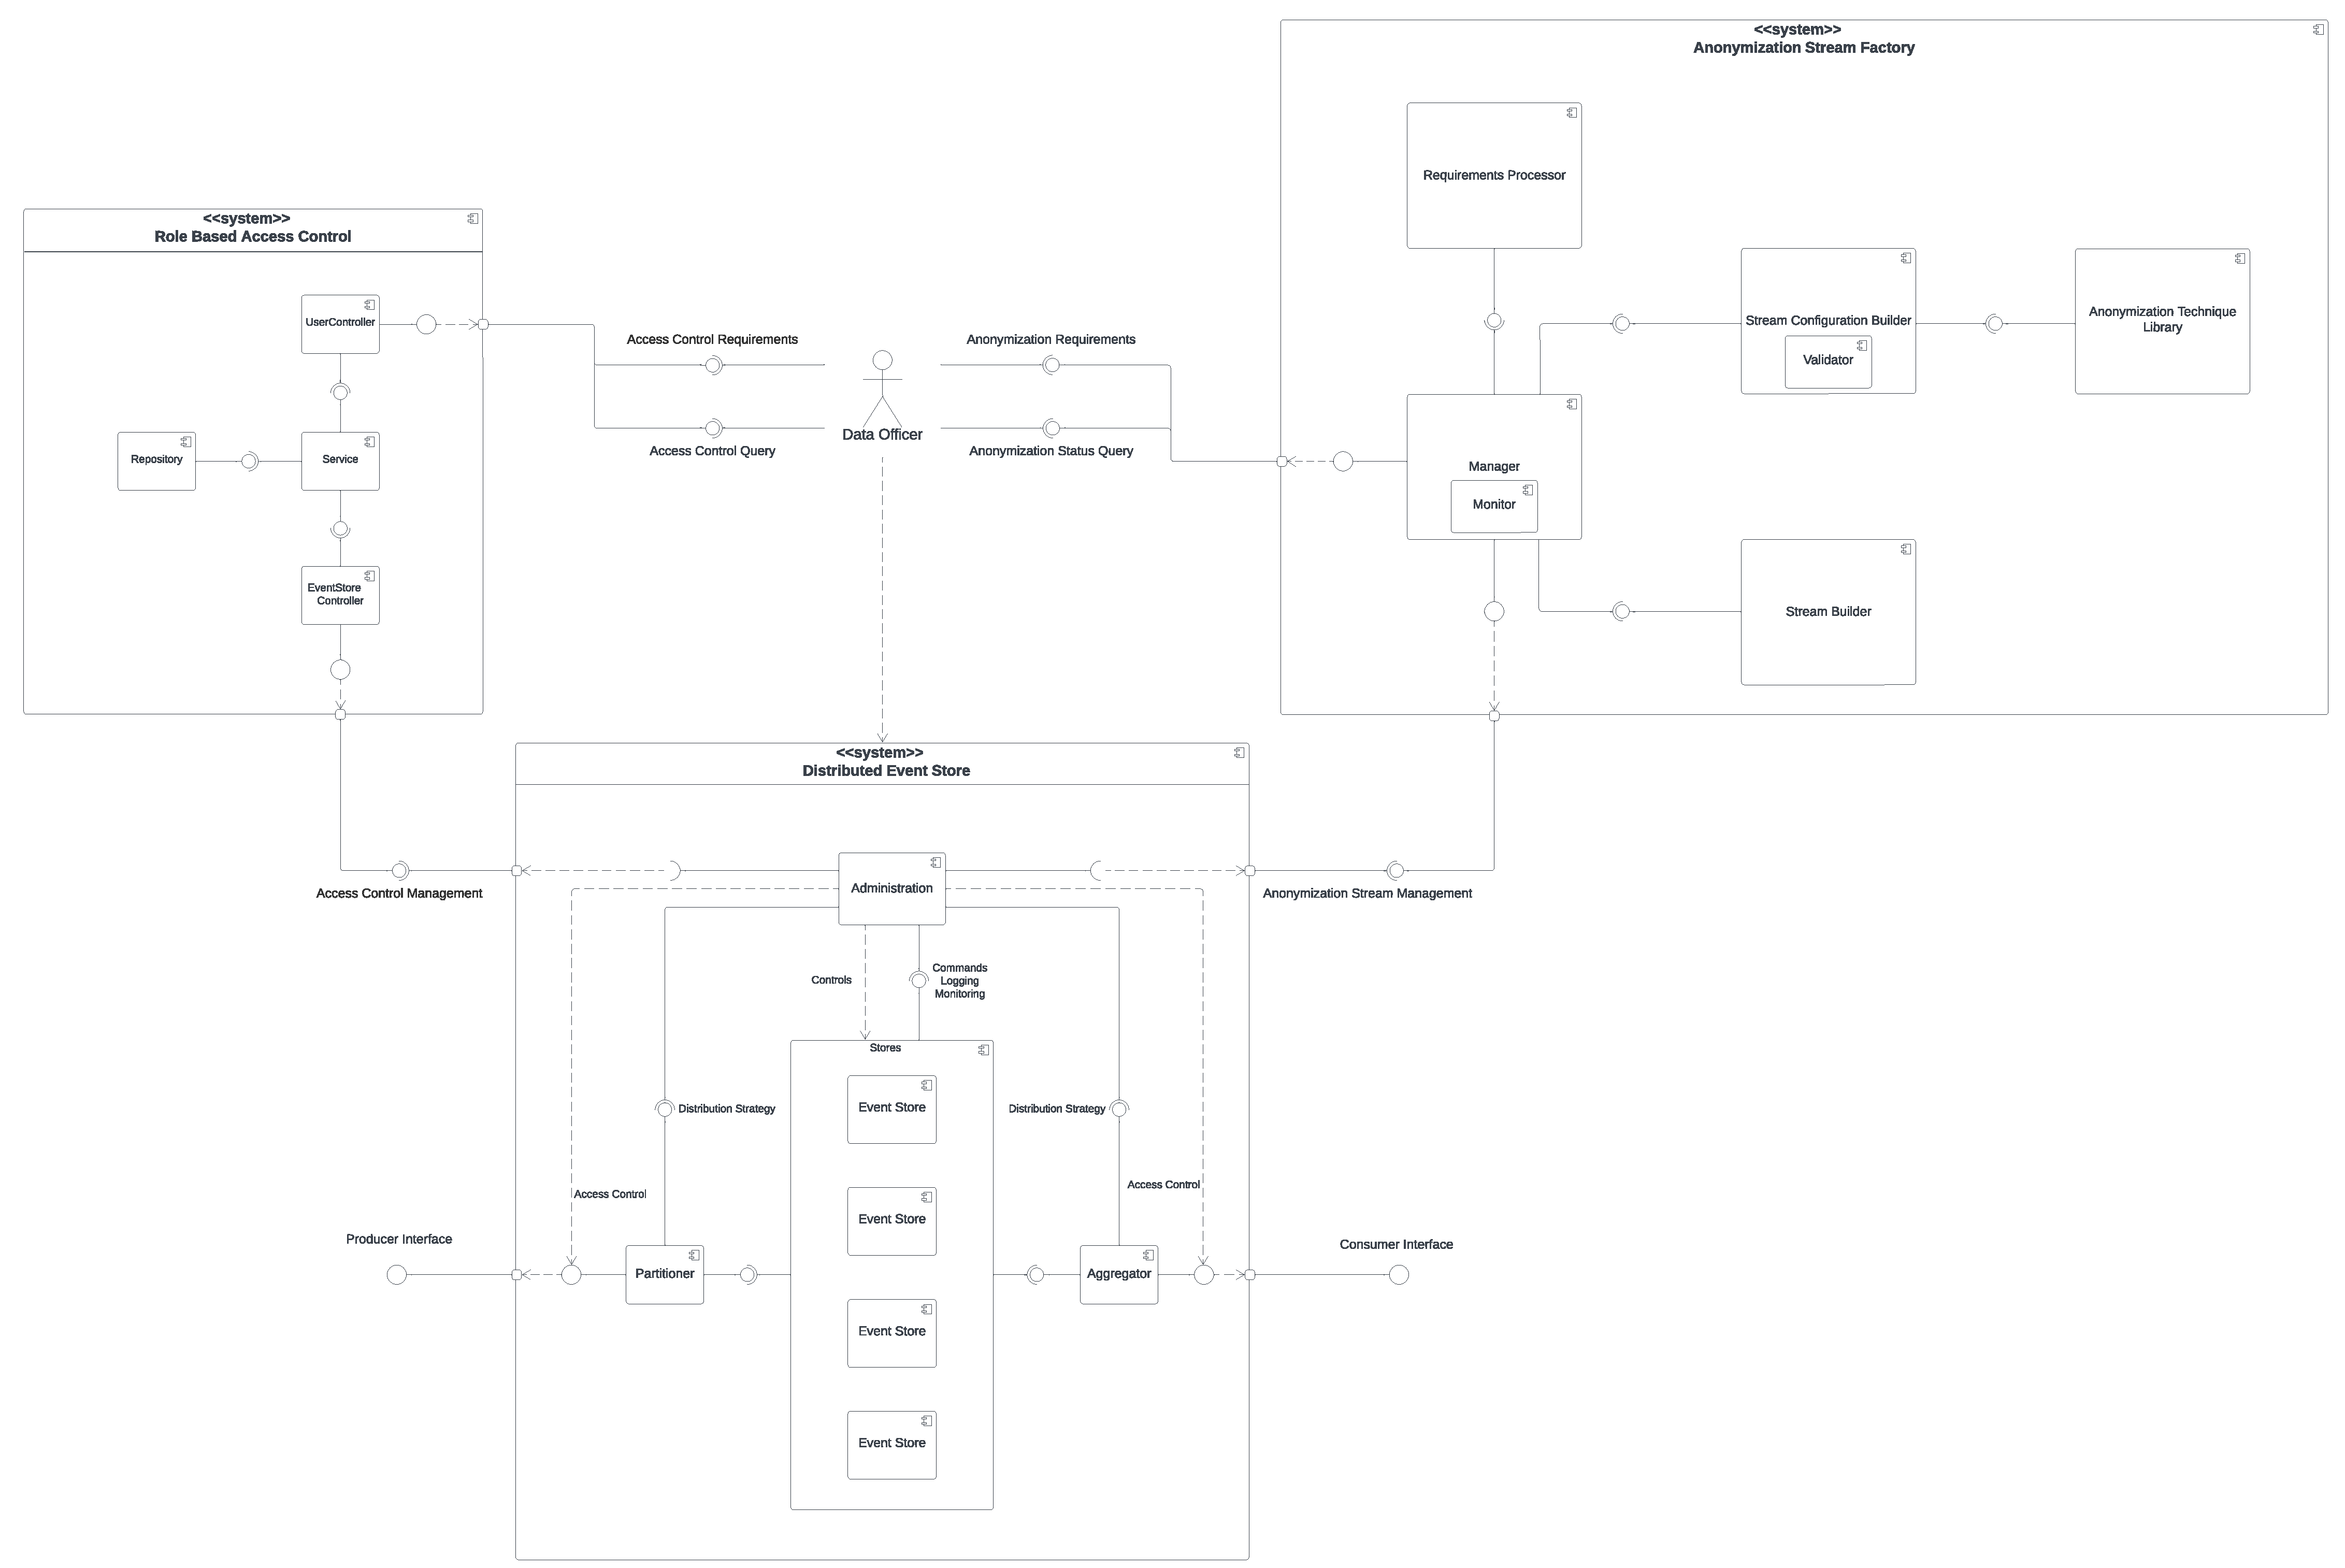
\includegraphics[width=\linewidth]{img/Complete_Component_Diagram.pdf}
    \caption{Full UML Component Diagram for the system as a whole.}
    \label{app:component_diagram}
\end{sidewaysfigure}


\addchap{Appendix B. Extended Version of the Experimental Results}


\end{document}
